\section{Results and discussion}
\label{sec:experiment}

\subsection{Impact of stochastic decomposition}
To assess the impact of the underlying stochastic decomposition method on PMAO, we create four variants of PMAO and PASTA (Table~\ref{tab:variants}). In particular, we vary the number of iterations and consider both \textit{mincluster} based (i.e., the default for PASTA) and stochastic decomposition. Increasing the iteration potentially intensifies the effect of the stochastic decomposition in PMAO framework. In Tables~\ref{tab:pmao-variants-a},  \ref{tab:pmao-variants-b}, we report the best FN rates among the 30 solutions generated by PMAO variants for datasets under set A and B, respectively; lower (i.e., better) FN rate values are marked with a darker shade.
%To assist in comparing the performance of four variants on each dataset, we mark the lower (i.e., better) FN rate values with a darker shade. 
We observe that the PMAO-3I-S and PMAO-8I-S columns contain more darker shades than PMAO-3I-D and PMAO-8I-D columns, which indicates the positive impact of stochastic decomposition on the performance of PMAO framework. To contrast among these variants, we apply the Friedman Aligned Ranks test~\cite{hodges2012rank} followed by complementary Holm’s post-hoc procedure~\cite{holm1979simple} on Tables~\ref{tab:pmao-variants-a},  \ref{tab:pmao-variants-b}, as recommended by~\cite{derrac2011practical, rodriguez-fdez2015stac} using 95\% confidence level. The results the summarized in Table~\ref{tab:test-pmao-variants}. The lower ranks of stochastic variants and significant difference between PMAO-3I-D and PMAO-8I-S suggest the effectiveness of stochastic decomposition. Note that PASTA uses three iterations by default, and most of its improvement is achieved in the first iteration. So, increasing iteration is not expected to improve PASTA output significantly. Moreover, stochastic decomposition makes sense in the context of MO principles as discussed earlier in Section~\ref{subsec:stocastic}. We have verified this by conducting similar analyses (Supplementary Tables~\ref{tab:pasta-variants-a}, \ref{tab:pasta-variants-b},  \ref{tab:test-pasta-variants}) based on four PASTA variants. The PASTA-3I-S variant does not get ample opportunity to leverage the stochastic decomposition due to its single execution.
In contrast, the PMAO-3I-S variant executes that 30 times on different search spaces defined by the weight vectors. We find no significant difference between any pair of PASTA variants as expected (Supplementary Table~\ref{tab:test-pasta-variants}), and PASTA-8I-D seems to be the best variant (more darker shades). In the subsequent sections, we use the PMAO-8I-S and the PASTA-8I-D variants for a fair comparison. 
%to ensure a level playing ground.

% Table generated by Excel2LaTeX from sheet 'small latex table'
\begin{table}[!htbp]
  \centering
  \caption{PMAO and PASTA variants based on iteration count and guide tree decomposition strategy.}
    \begin{tabular}{c|l|r|l}
    \multicolumn{1}{l|}{Method} & Variant & \multicolumn{1}{l|}{Iteration} & Tree decomposition [b]\\
    \hline
    \multirow{4}{*}{PMAO} & PMAO-3I-D  & 3     & Default (\textit{mincluster}) \\
\cline{2-4}          & 	PMAO-8I-D  & 8     & Default (\textit{mincluster}) \\
\cline{2-4}          & PMAO-3I-S  & 3     & Stochastic \\
\cline{2-4}          & PMAO-8I-S  & 8     & Stochastic\\
\hline \hline
    \multirow{4}{*}{PASTA} & PMAO-3I-D  & 3     & Default (\textit{mincluster}) \\
\cline{2-4}          & PASTA-8I-D  & 8     & Default (\textit{mincluster}) \\
\cline{2-4}          & PASTA-3I-S  & 3     & Stochastic \\
\cline{2-4}          & PASTA-8I-S  & 8     & Stochastic\\
    \hline
    \end{tabular}%
  \label{tab:variants}%
\end{table}%


% Table generated by Excel2LaTeX from sheet 'Sheet4'
\begin{table}[!htbp]
	%\centering
	\caption{Best FN rate achieved by the four variants of PMAO for each dataset in set A. On each row, the lower (better) FN rates are marked with darker shade.}
	\begin{tabular}{|l|r|r|r|r|}
		\hline
		\multirow{2}{*}{Dataset} & \multicolumn{4}{c|}{Best FN rates achieved by PMAO variants} \\
		\cline{2-5}          & PMAO-3I-D & PMAO-8I-D & PMAO-3I-S & PMAO-8I-S \\
		\hline
		BB11005 & \cellcolor[rgb]{ .988,  1,  .992}0.18 & \cellcolor[rgb]{ .384,  .745,  .478}0.09 & \cellcolor[rgb]{ .384,  .745,  .478}0.09 & \cellcolor[rgb]{ .384,  .745,  .478}0.09 \\
		\hline
		BB11018 & \cellcolor[rgb]{ .988,  1,  .992}0.27 & \cellcolor[rgb]{ .384,  .745,  .478}0.18 & \cellcolor[rgb]{ .384,  .745,  .478}0.18 & \cellcolor[rgb]{ .384,  .745,  .478}0.18 \\
		\hline
		BB11033 & \cellcolor[rgb]{ .988,  1,  .992}0.38 & \cellcolor[rgb]{ .988,  1,  .992}0.38 & \cellcolor[rgb]{ .988,  1,  .992}0.38 & \cellcolor[rgb]{ .988,  1,  .992}0.38 \\
		\hline
		BB11020 & \cellcolor[rgb]{ .988,  1,  .992}0.33 & \cellcolor[rgb]{ .988,  1,  .992}0.33 & \cellcolor[rgb]{ .988,  1,  .992}0.33 & \cellcolor[rgb]{ .988,  1,  .992}0.33 \\
		\hline
		BB12001 & \cellcolor[rgb]{ .988,  1,  .992}0.13 & \cellcolor[rgb]{ .988,  1,  .992}0.13 & \cellcolor[rgb]{ .988,  1,  .992}0.13 & \cellcolor[rgb]{ .988,  1,  .992}0.13 \\
		\hline
		BB12013 & \cellcolor[rgb]{ .384,  .745,  .478}0.00 & \cellcolor[rgb]{ .988,  1,  .992}0.20 & \cellcolor[rgb]{ .384,  .745,  .478}0.00 & \cellcolor[rgb]{ .988,  1,  .992}0.20 \\
		\hline
		BB12022 & \cellcolor[rgb]{ .988,  1,  .992}0.00 & \cellcolor[rgb]{ .988,  1,  .992}0.00 & \cellcolor[rgb]{ .988,  1,  .992}0.00 & \cellcolor[rgb]{ .988,  1,  .992}0.00 \\
		\hline
		BB12035 & \cellcolor[rgb]{ .988,  1,  .992}0.04 & \cellcolor[rgb]{ .384,  .745,  .478}0.00 & \cellcolor[rgb]{ .988,  1,  .992}0.04 & \cellcolor[rgb]{ .988,  1,  .992}0.04 \\
		\hline
		BB12044 & \cellcolor[rgb]{ .988,  1,  .992}0.38 & \cellcolor[rgb]{ .988,  1,  .992}0.38 & \cellcolor[rgb]{ .988,  1,  .992}0.38 & \cellcolor[rgb]{ .988,  1,  .992}0.38 \\
		\hline
		BB20001 & \cellcolor[rgb]{ .384,  .745,  .478}0.23 & \cellcolor[rgb]{ .988,  1,  .992}0.46 & \cellcolor[rgb]{ .384,  .745,  .478}0.23 & \cellcolor[rgb]{ .384,  .745,  .478}0.23 \\
		\hline
		BB20010 & \cellcolor[rgb]{ .988,  1,  .992}0.31 & \cellcolor[rgb]{ .988,  1,  .992}0.31 & \cellcolor[rgb]{ .384,  .745,  .478}0.08 & \cellcolor[rgb]{ .384,  .745,  .478}0.08 \\
		\hline
		BB20022 & \cellcolor[rgb]{ .988,  1,  .992}0.11 & \cellcolor[rgb]{ .988,  1,  .992}0.11 & \cellcolor[rgb]{ .988,  1,  .992}0.11 & \cellcolor[rgb]{ .384,  .745,  .478}0.09 \\
		\hline
		BB20033 & \cellcolor[rgb]{ .988,  1,  .992}0.36 & \cellcolor[rgb]{ .988,  1,  .992}0.36 & \cellcolor[rgb]{ .988,  1,  .992}0.36 & \cellcolor[rgb]{ .384,  .745,  .478}0.24 \\
		\hline
		BB20041 & \cellcolor[rgb]{ .988,  1,  .992}0.33 & \cellcolor[rgb]{ .584,  .827,  .647}0.29 & \cellcolor[rgb]{ .384,  .745,  .478}0.27 & \cellcolor[rgb]{ .988,  1,  .992}0.33 \\
		\hline
		BB30002 & \cellcolor[rgb]{ .988,  1,  .992}0.32 & \cellcolor[rgb]{ .988,  1,  .992}0.32 & \cellcolor[rgb]{ .384,  .745,  .478}0.14 & \cellcolor[rgb]{ .502,  .792,  .58}0.18 \\
		\hline
		BB30008 & \cellcolor[rgb]{ .533,  .808,  .604}0.24 & \cellcolor[rgb]{ .988,  1,  .992}0.33 & \cellcolor[rgb]{ .835,  .933,  .863}0.30 & \cellcolor[rgb]{ .384,  .745,  .478}0.21 \\
		\hline
		BB30015 & \cellcolor[rgb]{ .988,  1,  .992}0.17 & \cellcolor[rgb]{ .988,  1,  .992}0.17 & \cellcolor[rgb]{ .988,  1,  .992}0.17 & \cellcolor[rgb]{ .988,  1,  .992}0.17 \\
		\hline
		BB30022 & \cellcolor[rgb]{ .682,  .871,  .733}0.48 & \cellcolor[rgb]{ .682,  .871,  .733}0.48 & \cellcolor[rgb]{ .988,  1,  .992}0.49 & \cellcolor[rgb]{ .384,  .745,  .478}0.46 \\
		\hline
		BB40001 & \cellcolor[rgb]{ .988,  1,  .992}0.48 & \cellcolor[rgb]{ .784,  .914,  .82}0.44 & \cellcolor[rgb]{ .988,  1,  .992}0.48 & \cellcolor[rgb]{ .384,  .745,  .478}0.36 \\
		\hline
		BB40013 & \cellcolor[rgb]{ .988,  1,  .992}0.31 & \cellcolor[rgb]{ .988,  1,  .992}0.31 & \cellcolor[rgb]{ .988,  1,  .992}0.31 & \cellcolor[rgb]{ .384,  .745,  .478}0.25 \\
		\hline
		BB40025 & \cellcolor[rgb]{ .988,  1,  .992}0.00 & \cellcolor[rgb]{ .988,  1,  .992}0.00 & \cellcolor[rgb]{ .988,  1,  .992}0.00 & \cellcolor[rgb]{ .988,  1,  .992}0.00 \\
		\hline
		BB40038 & \cellcolor[rgb]{ .988,  1,  .992}0.10 & \cellcolor[rgb]{ .988,  1,  .992}0.10 & \cellcolor[rgb]{ .988,  1,  .992}0.10 & \cellcolor[rgb]{ .988,  1,  .992}0.10 \\
		\hline
		BB40048 & \cellcolor[rgb]{ .988,  1,  .992}0.29 & \cellcolor[rgb]{ .988,  1,  .992}0.29 & \cellcolor[rgb]{ .384,  .745,  .478}0.21 & \cellcolor[rgb]{ .988,  1,  .992}0.29 \\
		\hline
		BB50001 & \cellcolor[rgb]{ .988,  1,  .992}0.29 & \cellcolor[rgb]{ .988,  1,  .992}0.29 & \cellcolor[rgb]{ .988,  1,  .992}0.29 & \cellcolor[rgb]{ .988,  1,  .992}0.29 \\
		\hline
		BB50005 & \cellcolor[rgb]{ .686,  .871,  .733}0.25 & \cellcolor[rgb]{ .988,  1,  .992}0.38 & \cellcolor[rgb]{ .384,  .745,  .478}0.13 & \cellcolor[rgb]{ .686,  .871,  .733}0.25 \\
		\hline
		BB50010 & \cellcolor[rgb]{ .988,  1,  .992}0.07 & \cellcolor[rgb]{ .384,  .745,  .478}0.00 & \cellcolor[rgb]{ .384,  .745,  .478}0.00 & \cellcolor[rgb]{ .384,  .745,  .478}0.00 \\
		\hline
		BB50016 & \cellcolor[rgb]{ .682,  .871,  .733}0.13 & \cellcolor[rgb]{ .988,  1,  .992}0.20 & \cellcolor[rgb]{ .384,  .745,  .478}0.07 & \cellcolor[rgb]{ .384,  .745,  .478}0.07 \\
		\hline
	\end{tabular}%
	\label{tab:pmao-variants-a}%
\end{table}%

% Table generated by Excel2LaTeX from sheet 'Sheet4'
\begin{table}[!htbp]
	\small
	%\centering
	\caption{Best FN rate achieved by the four variants of PMAO for each dataset in set B. On each row, the lower (better) FN rates are marked with darker shade.}
	\begin{tabular}{|l|r|r|r|r|}
		\hline
		\multirow{2}{*}{Dataset} & \multicolumn{4}{c|}{Best FN rates achieved by PMAO variants} \\
		\cline{2-5}          & \multicolumn{1}{l|}{PMAO-3I-D} & \multicolumn{1}{l|}{PMAO-8I-D} & \multicolumn{1}{l|}{PMAO-3I-S} & \multicolumn{1}{l|}{PMAO-8I-S} \\
		\hline
		BB11007 & \cellcolor[rgb]{ .384,  .745,  .478}0.33 & \cellcolor[rgb]{ .384,  .745,  .478}0.33 & \cellcolor[rgb]{ .988,  1,  .992}0.50 & \cellcolor[rgb]{ .384,  .745,  .478}0.33 \\
		\hline
		BB11034 & \cellcolor[rgb]{ .988,  1,  .992}0.20 & \cellcolor[rgb]{ .384,  .745,  .478}0.00 & \cellcolor[rgb]{ .988,  1,  .992}0.20 & \cellcolor[rgb]{ .988,  1,  .992}0.20 \\
		\hline
		BB11038 & \cellcolor[rgb]{ .384,  .745,  .478}0.00 & \cellcolor[rgb]{ .384,  .745,  .478}0.00 & \cellcolor[rgb]{ .988,  1,  .992}0.40 & \cellcolor[rgb]{ .384,  .745,  .478}0.00 \\
		\hline
		BB11019 & \cellcolor[rgb]{ .988,  1,  .992}0.14 & \cellcolor[rgb]{ .988,  1,  .992}0.14 & \cellcolor[rgb]{ .988,  1,  .992}0.14 & \cellcolor[rgb]{ .988,  1,  .992}0.14 \\
		\hline
		BB12005 & \cellcolor[rgb]{ .988,  1,  .992}0.33 & \cellcolor[rgb]{ .988,  1,  .992}0.33 & \cellcolor[rgb]{ .988,  1,  .992}0.33 & \cellcolor[rgb]{ .988,  1,  .992}0.33 \\
		\hline
		BB12029 & \cellcolor[rgb]{ .988,  1,  .992}0.44 & \cellcolor[rgb]{ .988,  1,  .992}0.44 & \cellcolor[rgb]{ .384,  .745,  .478}0.33 & \cellcolor[rgb]{ .384,  .745,  .478}0.33 \\
		\hline
		BB12026 & \cellcolor[rgb]{ .384,  .745,  .478}0.27 & \cellcolor[rgb]{ .384,  .745,  .478}0.27 & \cellcolor[rgb]{ .384,  .745,  .478}0.27 & \cellcolor[rgb]{ .988,  1,  .992}0.33 \\
		\hline
		BB12037 & \cellcolor[rgb]{ .988,  1,  .992}0.10 & \cellcolor[rgb]{ .988,  1,  .992}0.10 & \cellcolor[rgb]{ .988,  1,  .992}0.10 & \cellcolor[rgb]{ .988,  1,  .992}0.10 \\
		\hline
		BB20002 & \cellcolor[rgb]{ .686,  .871,  .733}0.53 & \cellcolor[rgb]{ .384,  .745,  .478}0.47 & \cellcolor[rgb]{ .988,  1,  .992}0.59 & \cellcolor[rgb]{ .686,  .871,  .733}0.53 \\
		\hline
		BB20012 & \cellcolor[rgb]{ .988,  1,  .992}0.29 & \cellcolor[rgb]{ .745,  .894,  .784}0.21 & \cellcolor[rgb]{ .745,  .894,  .784}0.21 & \cellcolor[rgb]{ .384,  .745,  .478}0.08 \\
		\hline
		BB20030 & \cellcolor[rgb]{ .988,  1,  .992}0.64 & \cellcolor[rgb]{ .384,  .745,  .478}0.50 & \cellcolor[rgb]{ .988,  1,  .992}0.64 & \cellcolor[rgb]{ .988,  1,  .992}0.64 \\
		\hline
		BB20037 & \cellcolor[rgb]{ .988,  1,  .992}0.13 & \cellcolor[rgb]{ .988,  1,  .992}0.13 & \cellcolor[rgb]{ .988,  1,  .992}0.13 & \cellcolor[rgb]{ .988,  1,  .992}0.13 \\
		\hline
		BB30003 & \cellcolor[rgb]{ .988,  1,  .992}0.27 & \cellcolor[rgb]{ .384,  .745,  .478}0.25 & \cellcolor[rgb]{ .682,  .871,  .733}0.26 & \cellcolor[rgb]{ .682,  .871,  .733}0.26 \\
		\hline
		BB30021 & \cellcolor[rgb]{ .729,  .89,  .769}0.30 & \cellcolor[rgb]{ .816,  .925,  .843}0.31 & \cellcolor[rgb]{ .384,  .745,  .478}0.27 & \cellcolor[rgb]{ .988,  1,  .992}0.32 \\
		\hline
		BB30026 & \cellcolor[rgb]{ .384,  .745,  .478}0.15 & \cellcolor[rgb]{ .384,  .745,  .478}0.15 & \cellcolor[rgb]{ .988,  1,  .992}0.17 & \cellcolor[rgb]{ .384,  .745,  .478}0.15 \\
		\hline
		BB30011 & \cellcolor[rgb]{ .988,  1,  .992}0.32 & \cellcolor[rgb]{ .384,  .745,  .478}0.31 & \cellcolor[rgb]{ .384,  .745,  .478}0.31 & \cellcolor[rgb]{ .384,  .745,  .478}0.31 \\
		\hline
		BB40009 & \cellcolor[rgb]{ .988,  1,  .992}0.13 & \cellcolor[rgb]{ .988,  1,  .992}0.13 & \cellcolor[rgb]{ .988,  1,  .992}0.13 & \cellcolor[rgb]{ .988,  1,  .992}0.13 \\
		\hline
		BB40019 & \cellcolor[rgb]{ .988,  1,  .992}0.29 & \cellcolor[rgb]{ .988,  1,  .992}0.29 & \cellcolor[rgb]{ .384,  .745,  .478}0.14 & \cellcolor[rgb]{ .988,  1,  .992}0.29 \\
		\hline
		BB40033 & \cellcolor[rgb]{ .988,  1,  .992}0.06 & \cellcolor[rgb]{ .988,  1,  .992}0.06 & \cellcolor[rgb]{ .988,  1,  .992}0.06 & \cellcolor[rgb]{ .988,  1,  .992}0.06 \\
		\hline
		BB40006 & \cellcolor[rgb]{ .988,  1,  .992}0.00 & \cellcolor[rgb]{ .988,  1,  .992}0.00 & \cellcolor[rgb]{ .988,  1,  .992}0.00 & \cellcolor[rgb]{ .988,  1,  .992}0.00 \\
		\hline
		BB50002 & \cellcolor[rgb]{ .384,  .745,  .478}0.40 & \cellcolor[rgb]{ .988,  1,  .992}0.50 & \cellcolor[rgb]{ .988,  1,  .992}0.50 & \cellcolor[rgb]{ .384,  .745,  .478}0.40 \\
		\hline
		BB50009 & \cellcolor[rgb]{ .988,  1,  .992}0.08 & \cellcolor[rgb]{ .988,  1,  .992}0.08 & \cellcolor[rgb]{ .988,  1,  .992}0.08 & \cellcolor[rgb]{ .988,  1,  .992}0.08 \\
		\hline
		BB50014 & \cellcolor[rgb]{ .988,  1,  .992}0.41 & \cellcolor[rgb]{ .988,  1,  .992}0.41 & \cellcolor[rgb]{ .988,  1,  .992}0.41 & \cellcolor[rgb]{ .384,  .745,  .478}0.26 \\
		\hline
		BB50006 & \cellcolor[rgb]{ .988,  1,  .992}0.16 & \cellcolor[rgb]{ .988,  1,  .992}0.16 & \cellcolor[rgb]{ .988,  1,  .992}0.16 & \cellcolor[rgb]{ .384,  .745,  .478}0.12 \\
		\hline
	\end{tabular}%
	\label{tab:pmao-variants-b}%
\end{table}%

% Table generated by Excel2LaTeX from sheet 'stat test'
\begin{table}[!htbp]
	\small
	\caption{\underline{Friedman Aligned Ranks test (Column 2):} Friedman Aligned ranks (lower is better) of the four variants of PMAO based on Table~\ref{tab:pmao-variants-a},  \ref{tab:pmao-variants-b}. We also show the computed statistics and corresponding $ p $-value. 
		\underline{Holm's post-hoc procedure (Columns 3 - 6):} Comparison among the PMAO variants using the Holm's post-hoc procedures. Each entry shows the adjusted $p$-value which indicates the significance of the difference in performance between two methods.}
	\begin{tabular}{|l|r||c|c|c|c|}
		\hline
		\multicolumn{1}{|c|}{1} & \multicolumn{1}{c||}{2} & \multicolumn{1}{c|}{3} & \multicolumn{1}{c|}{4} & \multicolumn{1}{c|}{5} & 6 \\
		\hline
		\multirow{2}{*}{\makecell{PMAO\\ variants}} & \multirow{2}{*}{\makecell{Friedman\\Aligned rank*}} & \multicolumn{4}{c|}{Holm's adjusted $p$-value} \\
		\cline{3-6}          &       & 8I-S & 3I-S & 8I-D & 3I-D \\
		\hline
		8I-S & 82.3137 & \multicolumn{1}{c|}{-} & \multicolumn{1}{r|}{0.4032} & \multicolumn{1}{r|}{0.1431} & \multicolumn{1}{r|}{\cellcolor[rgb]{ .384,  .745,  .478}0.0077} \\
		\hline
		3I-S & 99.8137 & \multicolumn{1}{r|}{0.4032} & \multicolumn{1}{c|}{-} & \multicolumn{1}{r|}{0.6038} & \multicolumn{1}{r|}{0.3387} \\
		\hline
		8I-D & 107.9020 & \multicolumn{1}{r|}{0.1431} & \multicolumn{1}{r|}{0.6038} & \multicolumn{1}{c|}{-} & \multicolumn{1}{r|}{0.6038} \\
		\hline
		3I-D & 119.9706 & \multicolumn{1}{r|}{\cellcolor[rgb]{ .384,  .745,  .478}0.0077} & \multicolumn{1}{r|}{0.3387} & \multicolumn{1}{r|}{0.6038} & - \\
		\hline
		*Statistic & 9.0393 & \multicolumn{4}{c|}{\multirow{2}{*}{N/A}} \\
		\cline{1-2}    *$p$-value & 0.0288 & \multicolumn{4}{c|}{} \\
		\hline
	\end{tabular}%
	\label{tab:test-pmao-variants}%
\end{table}%

\subsection{Comparison between PASTA and PMAO}
We compare the solutions generated by PMAO (8I-S variant) with the output of PASTA (8I-D variant) in terms of FN rate. In particular, we report the PASTA FN rate alongside the best FN rate achieved by PMAO in Table~\ref{tab:pmao-pasta-a} and \ref{tab:pmao-pasta-b} where the better values are marked with darker shades. Furthermore, to give an overall picture of the tree-space generated by the PMAO framework, we include the average FN rate and count of those PMAO solutions equivalent to or better than PASTA. Except for BB12035, in every case, PMAO has at least one solution better than or equivalent to PASTA. Note that there are several solutions better than PASTA in the tree-space comprising 30 solutions and in 39 cases out of 51, more than 10 solutions are better than PASTA. We find that the best FN rates of PMAO are clearly ahead of PASTA's FN rate. In several cases the improvement is more than 50\% (e.g., BB11020, Bb20001, BB20010, BB40028, BB50016, BB11038, BB12037, BB20012, BB40033, BB50009, etc.). These results demonstrate the advantages of PMAO over PASTA. 

We present similar results considering all BAliBASE 3.0 datasets in Supplementary Table~\ref{tab:pmao-pasta-all} wherein more than 10 solutions are better than PASTA in 174 cases out of 218, and in 47 cases, the improvement of FN rate is more than 50\%.
% Table generated by Excel2LaTeX from sheet 'stat-8I-30w-S'
\begin{table}[!htbp]
	\small
	%\centering
	\caption{Comparison of the 30 solutions generated by PMAO with respect to PASTA in terms of FN rate on set A datasets. For PMAO, we show the best FN rate along with the average FN rate 
		and count of its solutions better or equivalent to PASTA. The better values are marked with darker shade.}
	\begin{tabular}{|l|r|r|r||r|}
		\hline
		\multirow{2}{*}{Dataset} & \multirow{2}{*}{\makecell{PASTA\\FN rate}} & \multicolumn{3}{c|}{\makecell{PMAO solutions better \\or equivalent to PASTA}} \\
		\cline{3-5}          &       & \multicolumn{1}{l|}{Best FN} & \multicolumn{1}{l|}{Avg FN} & \multicolumn{1}{l|}{Count} \\
		\hline
		BB11005 & \cellcolor[rgb]{ .988,  .988,  1}0.55 & \cellcolor[rgb]{ .388,  .745,  .482}0.09 & \cellcolor[rgb]{ .753,  .894,  .8}0.37 & \cellcolor[rgb]{ .976,  .451,  .459}28 \\
		\hline
		BB11018 & \cellcolor[rgb]{ .988,  .988,  1}0.27 & \cellcolor[rgb]{ .388,  .745,  .482}0.18 & \cellcolor[rgb]{ .784,  .906,  .824}0.24 & \cellcolor[rgb]{ .988,  .875,  .886}6 \\
		\hline
		BB11033 & \cellcolor[rgb]{ .988,  .988,  1}0.38 & \cellcolor[rgb]{ .988,  .988,  1}0.38 & \cellcolor[rgb]{ .988,  .988,  1}0.38 & \cellcolor[rgb]{ .988,  .894,  .906}5 \\
		\hline
		BB11020 & \cellcolor[rgb]{ .988,  .988,  1}0.83 & \cellcolor[rgb]{ .388,  .745,  .482}0.33 & \cellcolor[rgb]{ .733,  .882,  .78}0.62 & \cellcolor[rgb]{ .973,  .412,  .42}30 \\
		\hline
		BB12001 & \cellcolor[rgb]{ .988,  .988,  1}0.25 & \cellcolor[rgb]{ .388,  .745,  .482}0.13 & \cellcolor[rgb]{ .906,  .953,  .929}0.23 & \cellcolor[rgb]{ .98,  .702,  .71}15 \\
		\hline
		BB12013 & \cellcolor[rgb]{ .988,  .988,  1}0.20 & \cellcolor[rgb]{ .988,  .988,  1}0.20 & \cellcolor[rgb]{ .988,  .988,  1}0.20 & \cellcolor[rgb]{ .973,  .412,  .42}30 \\
		\hline
		BB12022 & \cellcolor[rgb]{ .988,  .988,  1}0.00 & \cellcolor[rgb]{ .988,  .988,  1}0.00 & \cellcolor[rgb]{ .988,  .988,  1}0.00 & \cellcolor[rgb]{ .976,  .51,  .518}25 \\
		\hline
		BB12035 & \cellcolor[rgb]{ .388,  .745,  .482}0.00  &   0.04    &   -    & \cellcolor[rgb]{ .988,  .988,  1}0 \\
		\hline
		BB12044 & \cellcolor[rgb]{ .988,  .988,  1}0.50 & \cellcolor[rgb]{ .388,  .745,  .482}0.38 & \cellcolor[rgb]{ .706,  .875,  .757}0.44 & \cellcolor[rgb]{ .973,  .412,  .42}30 \\
		\hline
		BB20001 & \cellcolor[rgb]{ .988,  .988,  1}0.54 & \cellcolor[rgb]{ .388,  .745,  .482}0.23 & \cellcolor[rgb]{ .843,  .929,  .875}0.46 & \cellcolor[rgb]{ .976,  .51,  .518}25 \\
		\hline
		BB20010 & \cellcolor[rgb]{ .988,  .988,  1}0.35 & \cellcolor[rgb]{ .388,  .745,  .482}0.08 & \cellcolor[rgb]{ .871,  .941,  .898}0.29 & \cellcolor[rgb]{ .976,  .549,  .557}23 \\
		\hline
		BB20022 & \cellcolor[rgb]{ .988,  .988,  1}0.11 & \cellcolor[rgb]{ .388,  .745,  .482}0.09 & \cellcolor[rgb]{ .925,  .961,  .945}0.11 & \cellcolor[rgb]{ .984,  .796,  .808}10 \\
		\hline
		BB20033 & \cellcolor[rgb]{ .988,  .988,  1}0.36 & \cellcolor[rgb]{ .388,  .745,  .482}0.24 & \cellcolor[rgb]{ .784,  .906,  .824}0.32 & \cellcolor[rgb]{ .984,  .816,  .827}9 \\
		\hline
		BB20041 & \cellcolor[rgb]{ .988,  .988,  1}0.38 & \cellcolor[rgb]{ .388,  .745,  .482}0.33 & \cellcolor[rgb]{ .8,  .91,  .835}0.36 & \cellcolor[rgb]{ .984,  .835,  .847}8 \\
		\hline
		BB30002 & \cellcolor[rgb]{ .988,  .988,  1}0.32 & \cellcolor[rgb]{ .388,  .745,  .482}0.18 & \cellcolor[rgb]{ .847,  .929,  .878}0.29 & \cellcolor[rgb]{ .98,  .702,  .71}15 \\
		\hline
		BB30008 & \cellcolor[rgb]{ .988,  .988,  1}0.33 & \cellcolor[rgb]{ .388,  .745,  .482}0.21 & \cellcolor[rgb]{ .878,  .941,  .906}0.31 & \cellcolor[rgb]{ .984,  .722,  .729}14 \\
		\hline
		BB30015 & \cellcolor[rgb]{ .988,  .988,  1}0.17 & \cellcolor[rgb]{ .988,  .988,  1}0.17 & \cellcolor[rgb]{ .988,  .988,  1}0.17 & \cellcolor[rgb]{ .984,  .761,  .769}12 \\
		\hline
		BB30022 & \cellcolor[rgb]{ .988,  .988,  1}0.51 & \cellcolor[rgb]{ .388,  .745,  .482}0.46 & \cellcolor[rgb]{ .902,  .953,  .925}0.50 & \cellcolor[rgb]{ .98,  .663,  .675}17 \\
		\hline
		BB40001 & \cellcolor[rgb]{ .988,  .988,  1}0.48 & \cellcolor[rgb]{ .388,  .745,  .482}0.36 & \cellcolor[rgb]{ .745,  .89,  .792}0.43 & \cellcolor[rgb]{ .984,  .796,  .808}10 \\
		\hline
		BB40013 & \cellcolor[rgb]{ .988,  .988,  1}0.38 & \cellcolor[rgb]{ .388,  .745,  .482}0.25 & \cellcolor[rgb]{ .753,  .89,  .796}0.33 & \cellcolor[rgb]{ .98,  .682,  .694}16 \\
		\hline
		BB40025 & \cellcolor[rgb]{ .988,  .988,  1}0.00 & \cellcolor[rgb]{ .988,  .988,  1}0.00 & \cellcolor[rgb]{ .988,  .988,  1}0.00 & \cellcolor[rgb]{ .98,  .569,  .576}22 \\
		\hline
		BB40038 & \cellcolor[rgb]{ .988,  .988,  1}0.25 & \cellcolor[rgb]{ .388,  .745,  .482}0.10 & \cellcolor[rgb]{ .788,  .906,  .827}0.20 & \cellcolor[rgb]{ .98,  .624,  .635}19 \\
		\hline
		BB40048 & \cellcolor[rgb]{ .988,  .988,  1}0.43 & \cellcolor[rgb]{ .388,  .745,  .482}0.29 & \cellcolor[rgb]{ .447,  .769,  .533}0.30 & \cellcolor[rgb]{ .973,  .412,  .42}30 \\
		\hline
		BB50001 & \cellcolor[rgb]{ .988,  .988,  1}0.29 & \cellcolor[rgb]{ .988,  .988,  1}0.29 & \cellcolor[rgb]{ .988,  .988,  1}0.29 & \cellcolor[rgb]{ .98,  .663,  .675}17 \\
		\hline
		BB50005 & \cellcolor[rgb]{ .988,  .988,  1}0.38 & \cellcolor[rgb]{ .388,  .745,  .482}0.25 & \cellcolor[rgb]{ .827,  .922,  .859}0.34 & \cellcolor[rgb]{ .973,  .412,  .42}30 \\
		\hline
		BB50010 & \cellcolor[rgb]{ .988,  .988,  1}0.00 & \cellcolor[rgb]{ .988,  .988,  1}0.00 & \cellcolor[rgb]{ .988,  .988,  1}0.00 & \cellcolor[rgb]{ .988,  .855,  .867}7 \\
		\hline
		BB50016 & \cellcolor[rgb]{ .988,  .988,  1}0.47 & \cellcolor[rgb]{ .388,  .745,  .482}0.07 & \cellcolor[rgb]{ .584,  .824,  .651}0.20 & \cellcolor[rgb]{ .976,  .451,  .459}28 \\
		\hline
	\end{tabular}%
	\label{tab:pmao-pasta-a}%
\end{table}%

% Table generated by Excel2LaTeX from sheet 'stat-8I-30w-S'
\begin{table}[!htbp]
	\small
	\caption{Comparison of the 30 solutions generated by PMAO with respect to PASTA in terms of FN rate on set B datasets. For PMAO, we show the best FN rate along with the average FN rate and count of its solutions better or equivalent to PASTA. The better values are marked with darker shade.}
	\begin{tabular}{|l|r|r|r||r|}
		\hline
		\multirow{2}{*}{Dataset} & \multirow{2}{*}{\makecell{PASTA\\FN rate}} & \multicolumn{3}{c|}{\makecell{PMAO solutions better \\or equivalent to PASTA}} \\
		\cline{3-5}          &       & \multicolumn{1}{l|}{Best FN} & \multicolumn{1}{l|}{Avg FN} & \multicolumn{1}{l|}{Count} \\
		\hline
		BB11007 & \cellcolor[rgb]{ .988,  1,  .992}0.50 & \cellcolor[rgb]{ .384,  .745,  .478}0.33 & \cellcolor[rgb]{ .906,  .965,  .922}0.48 & \cellcolor[rgb]{ .984,  .714,  .722}15 \\
		\hline
		BB11034 & \cellcolor[rgb]{ .988,  1,  .992}0.40 & \cellcolor[rgb]{ .384,  .745,  .478}0.20 & \cellcolor[rgb]{ .753,  .898,  .792}0.32 & \cellcolor[rgb]{ .98,  .651,  .663}18 \\
		\hline
		BB11038 & \cellcolor[rgb]{ .988,  1,  .992}0.40 & \cellcolor[rgb]{ .384,  .745,  .478}0.00 & \cellcolor[rgb]{ .937,  .976,  .949}0.37 & \cellcolor[rgb]{ .984,  .773,  .78}12 \\
		\hline
		BB11019 & \cellcolor[rgb]{ .988,  1,  .992}0.29 & \cellcolor[rgb]{ .384,  .745,  .478}0.14 & \cellcolor[rgb]{ .918,  .969,  .933}0.27 & \cellcolor[rgb]{ .976,  .475,  .482}27 \\
		\hline
		BB12005 & \cellcolor[rgb]{ .988,  1,  .992}0.33 & \cellcolor[rgb]{ .988,  1,  .992}0.33 & \cellcolor[rgb]{ .988,  1,  .992}0.33 & \cellcolor[rgb]{ .976,  .455,  .463}28 \\
		\hline
		BB12029 & \cellcolor[rgb]{ .988,  1,  .992}0.44 & \cellcolor[rgb]{ .384,  .745,  .478}0.33 & \cellcolor[rgb]{ .863,  .945,  .882}0.42 & \cellcolor[rgb]{ .976,  .435,  .443}29 \\
		\hline
		BB12026 & \cellcolor[rgb]{ .988,  1,  .992}0.53 & \cellcolor[rgb]{ .384,  .745,  .478}0.33 & \cellcolor[rgb]{ .816,  .925,  .847}0.48 & \cellcolor[rgb]{ .984,  .753,  .761}13 \\
		\hline
		BB12037 & \cellcolor[rgb]{ .988,  1,  .992}0.40 & \cellcolor[rgb]{ .384,  .745,  .478}0.10 & \cellcolor[rgb]{ .859,  .945,  .882}0.34 & \cellcolor[rgb]{ .988,  .851,  .863}8 \\
		\hline
		BB20002 & \cellcolor[rgb]{ .988,  1,  .992}0.65 & \cellcolor[rgb]{ .384,  .745,  .478}0.53 & \cellcolor[rgb]{ .835,  .933,  .863}0.62 & \cellcolor[rgb]{ .984,  .812,  .824}10 \\
		\hline
		BB20012 & \cellcolor[rgb]{ .988,  1,  .992}0.29 & \cellcolor[rgb]{ .384,  .745,  .478}0.08 & \cellcolor[rgb]{ .851,  .941,  .875}0.25 & \cellcolor[rgb]{ .976,  .494,  .502}26 \\
		\hline
		BB20030 & \cellcolor[rgb]{ .988,  1,  .992}0.64 & \cellcolor[rgb]{ .988,  1,  .992}0.64 & \cellcolor[rgb]{ .988,  1,  .992}0.64 & \cellcolor[rgb]{ .988,  .871,  .882}7 \\
		\hline
		BB20037 & \cellcolor[rgb]{ .988,  1,  .992}0.13 & \cellcolor[rgb]{ .988,  1,  .992}0.13 & \cellcolor[rgb]{ .988,  1,  .992}0.13 & \cellcolor[rgb]{ .988,  .988,  1}1 \\
		\hline
		BB30003 & \cellcolor[rgb]{ .988,  1,  .992}0.30 & \cellcolor[rgb]{ .384,  .745,  .478}0.26 & \cellcolor[rgb]{ .773,  .906,  .808}0.29 & \cellcolor[rgb]{ .98,  .573,  .58}22 \\
		\hline
		BB30021 & \cellcolor[rgb]{ .988,  1,  .992}0.36 & \cellcolor[rgb]{ .384,  .745,  .478}0.32 & \cellcolor[rgb]{ .663,  .863,  .714}0.34 & \cellcolor[rgb]{ .98,  .69,  .702}16 \\
		\hline
		BB30026 & \cellcolor[rgb]{ .988,  1,  .992}0.19 & \cellcolor[rgb]{ .384,  .745,  .478}0.15 & \cellcolor[rgb]{ .741,  .894,  .78}0.18 & \cellcolor[rgb]{ .984,  .831,  .843}9 \\
		\hline
		BB30011 & \cellcolor[rgb]{ .988,  1,  .992}0.35 & \cellcolor[rgb]{ .384,  .745,  .478}0.31 & \cellcolor[rgb]{ .894,  .957,  .91}0.35 & \cellcolor[rgb]{ .973,  .412,  .42}30 \\
		\hline
		BB40009 & \cellcolor[rgb]{ .988,  1,  .992}0.19 & \cellcolor[rgb]{ .384,  .745,  .478}0.13 & \cellcolor[rgb]{ .945,  .98,  .957}0.18 & \cellcolor[rgb]{ .984,  .714,  .722}15 \\
		\hline
		BB40019 & \cellcolor[rgb]{ .988,  1,  .992}0.43 & \cellcolor[rgb]{ .384,  .745,  .478}0.29 & \cellcolor[rgb]{ .725,  .886,  .769}0.37 & \cellcolor[rgb]{ .973,  .412,  .42}30 \\
		\hline
		BB40033 & \cellcolor[rgb]{ .988,  1,  .992}0.13 & \cellcolor[rgb]{ .384,  .745,  .478}0.06 & \cellcolor[rgb]{ .706,  .878,  .753}0.10 & \cellcolor[rgb]{ .976,  .455,  .463}28 \\
		\hline
		BB40006 & \cellcolor[rgb]{ .988,  1,  .992}0.00 & \cellcolor[rgb]{ .988,  1,  .992}0.00 & \cellcolor[rgb]{ .988,  1,  .992}0.00 & \cellcolor[rgb]{ .988,  .871,  .882}7 \\
		\hline
		BB50002 & \cellcolor[rgb]{ .988,  1,  .992}0.50 & \cellcolor[rgb]{ .384,  .745,  .478}0.40 & \cellcolor[rgb]{ .941,  .98,  .953}0.49 & \cellcolor[rgb]{ .984,  .733,  .741}14 \\
		\hline
		BB50009 & \cellcolor[rgb]{ .988,  1,  .992}0.24 & \cellcolor[rgb]{ .384,  .745,  .478}0.08 & \cellcolor[rgb]{ .788,  .914,  .82}0.19 & \cellcolor[rgb]{ .98,  .631,  .643}19 \\
		\hline
		BB50014 & \cellcolor[rgb]{ .988,  1,  .992}0.41 & \cellcolor[rgb]{ .384,  .745,  .478}0.26 & \cellcolor[rgb]{ .835,  .933,  .863}0.37 & \cellcolor[rgb]{ .984,  .812,  .824}10 \\
		\hline
		BB50006 & \cellcolor[rgb]{ .988,  1,  .992}0.21 & \cellcolor[rgb]{ .384,  .745,  .478}0.12 & \cellcolor[rgb]{ .725,  .886,  .769}0.17 & \cellcolor[rgb]{ .988,  .89,  .902}6 \\
		\hline
	\end{tabular}%
	\label{tab:pmao-pasta-b}%
\end{table}%

\subsubsection{Domain-specific measures and multiple objectives}
To illustrate a particular advantage of PMAO over PASTA, we plot the (ML score, FN rate) values of PASTA output and 30 solutions in the tree-space generated by PMAO in Figure~\ref{fig:ml-fn} for 10 arbitrary datasets. Such plot for all datasets of set A and set B are available in Supplementary Figures~\ref{fig:ml-fn-a}, \ref{fig:ml-fn-b}. We find several cases where a PMAO solution has a better ML score than PASTA but with a worse FN rate.  On the other hand, the best FN rate might correspond to an ML score much lower than PASTA. Similar observations can be shown for other objectives as well. These results illustrate the phenomena that, depending solely on a single optimization criterion (e.g., ML score by PASTA) may severely affect the accuracy. PMAO reduces such risk by employing many objectives.

\begin{figure*}[!htbp]%
	\begin{adjustwidth}{-1cm}{}
		\centering
		\subfloat[BB11018]{\includegraphics[width=0.22\textwidth]{PMAO-A/BB11018-fn-ml}}
		\subfloat[BB12001]{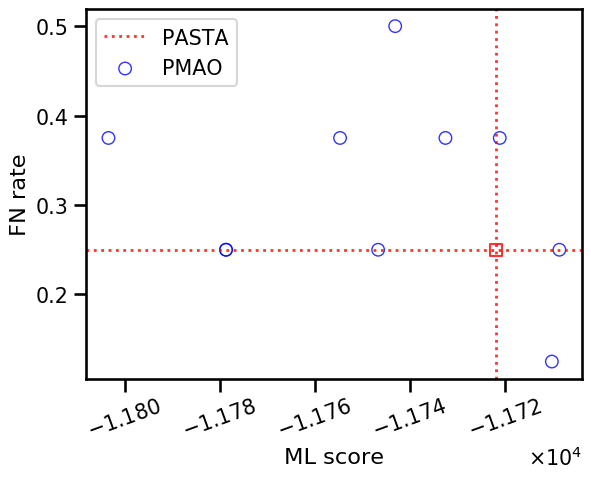
\includegraphics[width=0.22\textwidth]{PMAO-A/BB12001-fn-ml}}
		\subfloat[BB20010]{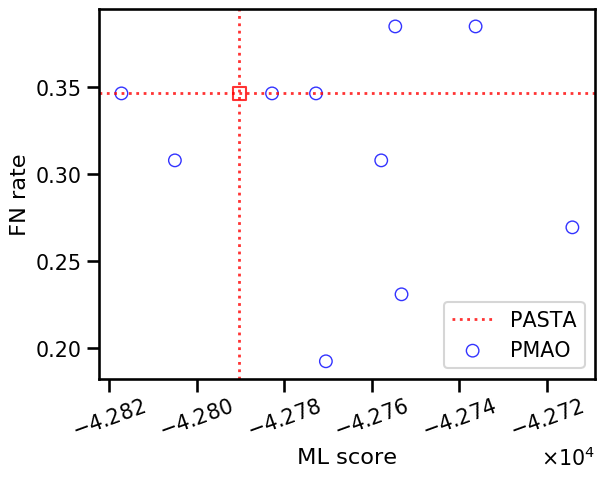
\includegraphics[width=0.22\textwidth]{PMAO-A/BB20010-fn-ml}}%
		\subfloat[BB20041]{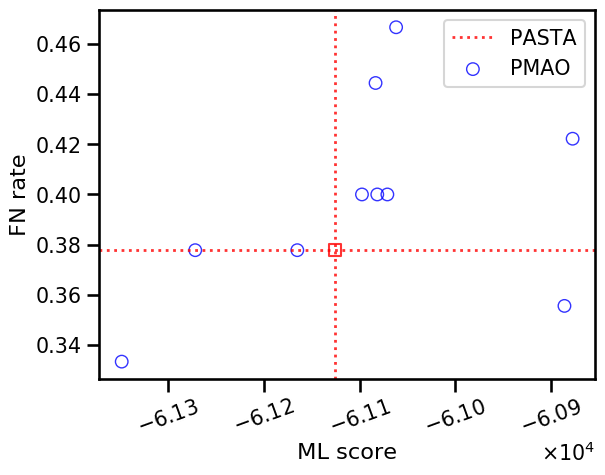
\includegraphics[width=0.22\textwidth]{PMAO-A/BB20041-fn-ml}}%
		\subfloat[BB30002]{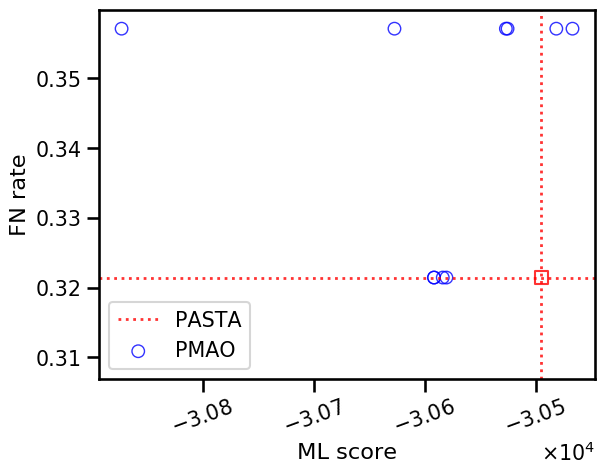
\includegraphics[width=0.22\textwidth]{PMAO-A/BB30002-fn-ml}}\\%
		\subfloat[BB30008]{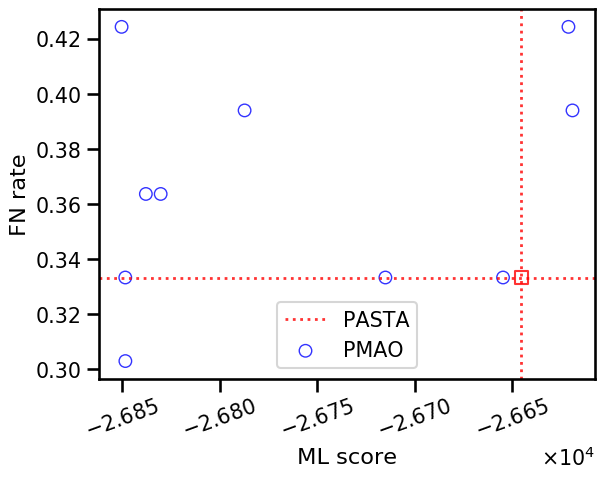
\includegraphics[width=0.22\textwidth]{PMAO-A/BB30008-fn-ml}}%
		\subfloat[BB40001]{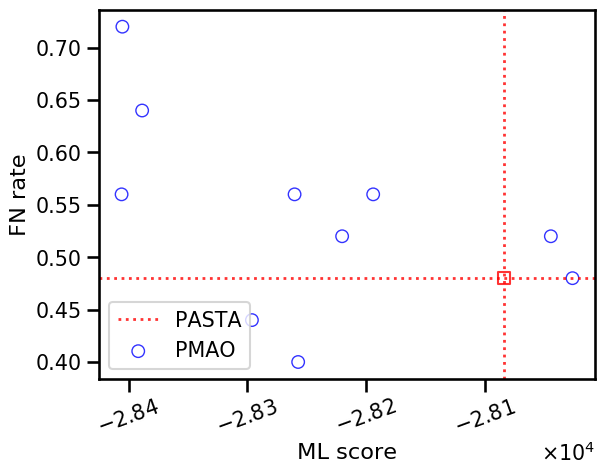
\includegraphics[width=0.22\textwidth]{PMAO-A/BB40001-fn-ml}}%
		\subfloat[BB40048]{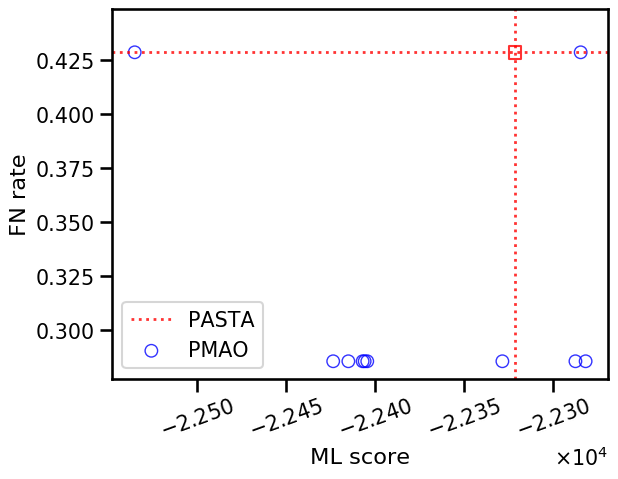
\includegraphics[width=0.22\textwidth]{PMAO-A/BB40048-fn-ml}}%
		\subfloat[BB50005]{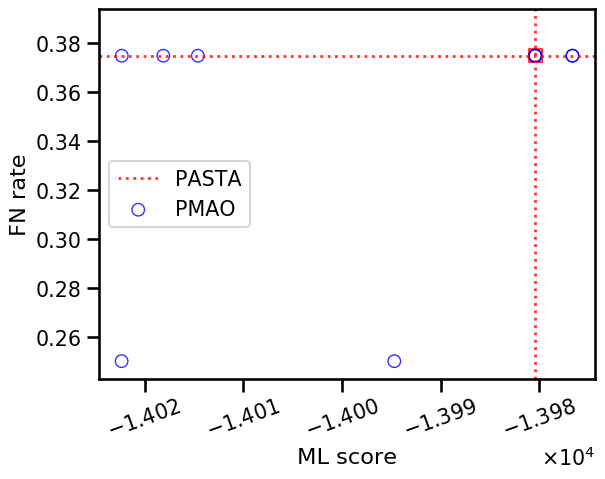
\includegraphics[width=0.22\textwidth]{PMAO-A/BB50005-fn-ml}}%	
		\subfloat[BB50016]{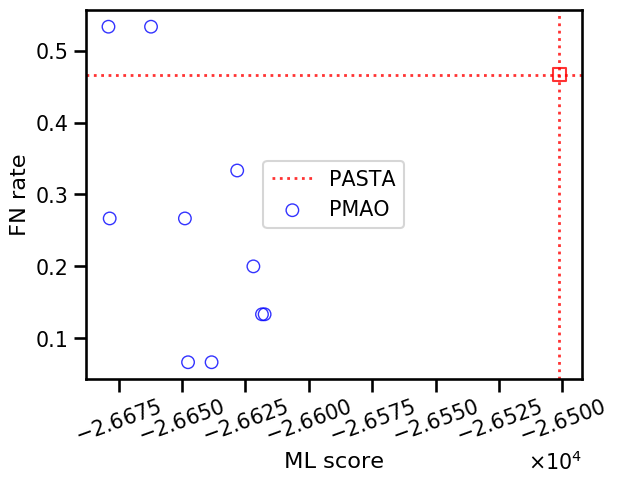
\includegraphics[width=0.22\textwidth]{PMAO-A/BB50016-fn-ml}}%
	\end{adjustwidth}
	\caption{Visualization of PASTA output and the 30 solutions generated by PMAO on 10 arbitrary datasets. The x-axis and y-axis represent ML score and FN rate respectively.}
	\label{fig:ml-fn}
\end{figure*}

\subsubsection{Contribution of MO strategy}
Now we examine the flexibility of decomposition-based MO strategy within the PMAO framework to address diverse characteristics varying across datasets. The weight vectors that resulted in better than or equivalent solutions than that of PASTA in four arbitrary datasets are illustrated in Figures~\ref{fig:good-weight}. Here each bar represents a weight vector along with its achieved FN rate.  Note that the weight vectors yielding the best FN rates vary across the datasets suggesting that the underlying MO mechanism is somewhat self-adapting itself according to the inherent characteristics of the dataset. This is all the more evident when the number of weight vectors is increased (please refer to Supplementary Table~\ref{tab:pmao-100}). Additionally, observe that nearly all weight vectors consist of two or more non-zero values indicating the contribution of multiple objectives in the overall optimization process. These justify our motivation for employing the MO approach incorporating multiple weight vectors, which ensures the robustness of PMAO framework to varying traits of the datasets. Similar plots for all datasets of set A and set B are available in Supplementary Figures~\ref{fig:good-weight-a}, \ref{fig:good-weight-b}.

\begin{figure}[!htbp]%
	\begin{adjustwidth}{-0.6cm}{}
		\centering
		\subfloat[BB12001]{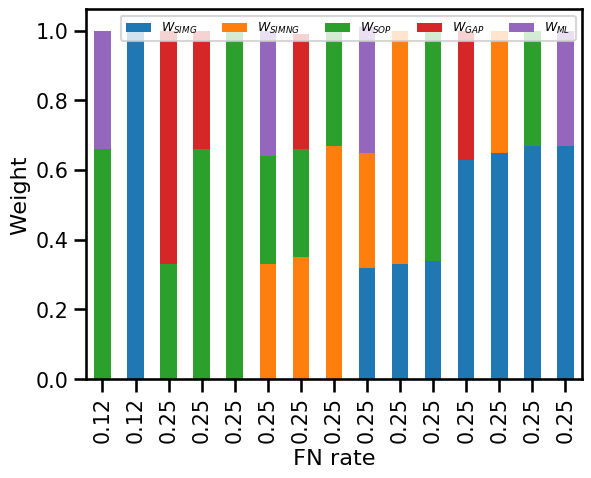
\includegraphics[width=0.25\textwidth]{weight-A/BB12001-good-weight}}
		%\subfloat[BB20010]{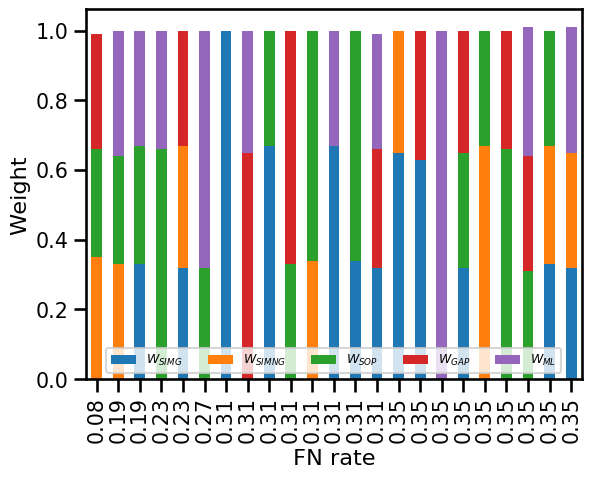
\includegraphics[width=0.22\textwidth]{weight-A/BB20010-good-weight}}%
		\subfloat[BB20041]{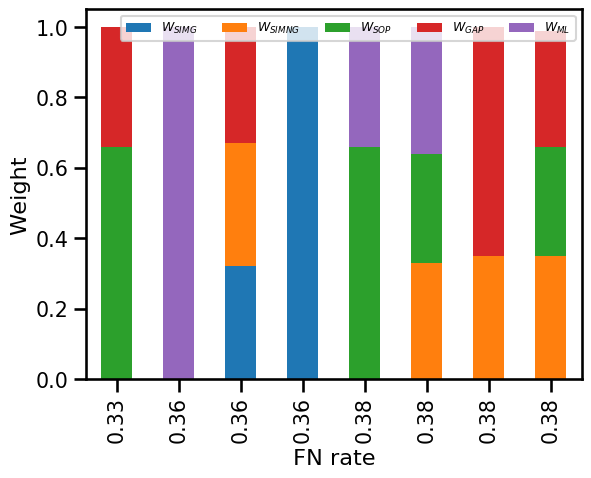
\includegraphics[width=0.25\textwidth]{weight-A/BB20041-good-weight}}\\
		%\subfloat[BB30002]{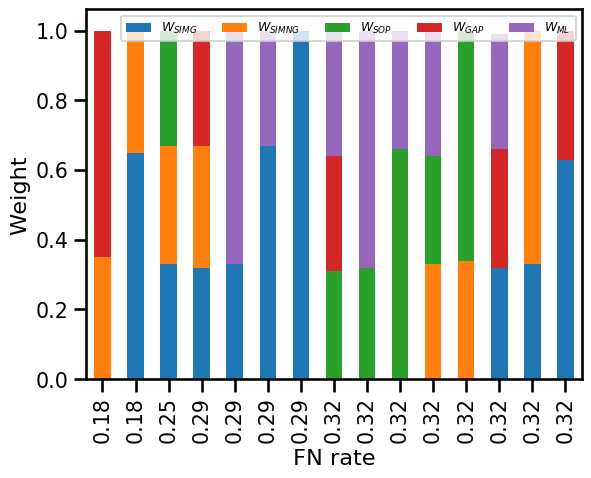
\includegraphics[width=0.22\textwidth]{weight-A/BB30002-good-weight}}\\%
		\subfloat[BB30008]{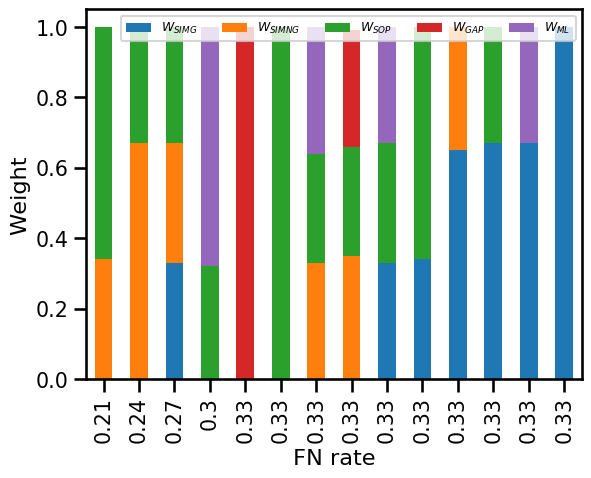
\includegraphics[width=0.25\textwidth]{weight-A/BB30008-good-weight}}%
		\subfloat[BB40001]{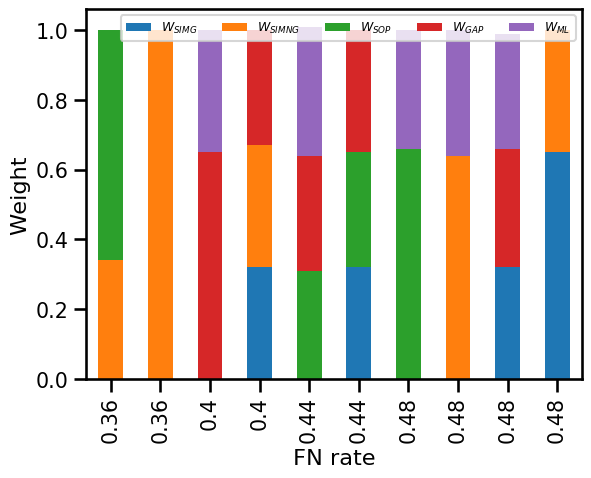
\includegraphics[width=0.25\textwidth]{weight-A/BB40001-good-weight}}%
	\end{adjustwidth}
	\caption{Visualization of weight vectors which lead PMAO to generate better or equivalent solutions to PASTA on four arbitrary datasets. The y-axis portrays the weight values and the x-axis marks the achieved FN rate. The weight vectors are sorted in ascending order based on the achieved FN rate. }
	\label{fig:good-weight}
\end{figure}


\subsection{Machine learning based detection of few wight vectors}
One awkward issue is that the MO optimization approaches usually provide a bunch of good quality solutions that are considered equivalent in the context of conflicting objectives under consideration. In MO terms, these are non-dominated solutions. However, from a practical point of view, it is often necessary to choose one of these as the final solution. While picking randomly could be an approach, but as experimental evidence suggests, if is unlikely that all solutions output by our PMAO framework for a particular input would be of the highest quality. So it is interesting to develop an approach that would help us choose the best one or at least a few top solutions from the output of PMAO. Such an approach would be of independent interest for other MO optimization scenarios as well.   

With the above backdrop, now we address whether it is possible to detect a few input weight vectors for PMAO, based on the features of the unaligned input sequences, such that the resultant smaller tree-space contains at least one high-quality tree. It can significantly reduce PAMO's computational cost as well as allow the domain expert to select the final solution with a manageable effort. We design a supervised regression-based pipeline to detect five promising weight vectors comprising the following steps to pursue this goal.
\begin{itemize}
	\item Step 1: Prepare training data to learn a regression model of the form, $FN\_rate = f(X)$, based on achieved FN rates by running PMAO with 30 input weight vectors on each dataset of set A. Here each 15D feature vector $X$ consists of the input 5D weight vector for PMAO plus 10 features (used by~\cite{rubio2018characteristic}) extracted from the unaligned protein sequences. More details can be found in Appendix~\ref{appendix:train_xgboost} of the Supplementary file.  
	\item Step 2: Fit an XGBoost regressor~\cite{chen2016xgboost}, a popular gradient tree boosting system, to the training data prepared in Step 1. For details please see Appendix~\ref{appendix:train_xgboost} in the Supplementary file. 
	%\item Step 3: 
	\item Step 3: Calculate 100 well-spaced 5D weight vectors (Supplementary Figure~\ref{fig:100-weights}) using the method of~\cite{ref_dirs_energy}. Then prepare a ($100 \times 15$) test data, for each dataset under set B, by appending 10 extracted features as mentioned in Step 1 (\cite{rubio2018characteristic}) to each of the 100 weight vectors. This step uses 100 weight vectors rather than 30, as they offer a wider range of promising weight vectors as suggested by Supplementary Table~\ref{tab:pmao-100}.
	\item Step 4: Predict the FN rate for each test feature vector formed in Step 4 using the model obtained in Step 2. 
	\item Step 5: For each dataset in set B, select the five test feature vectors having the most minor five predicted FN rates and output their respective weight vectors.
\end{itemize}

The five weight vectors detected in this way on four arbitrary datasets in set B are visualized in Figure~\ref{fig:some-good-weight-ml}. Supplementary Figure~\ref{fig:good-weight-ml} shows such weight vectors for all datasets. As a baseline, we randomly picked five weight vectors for each dataset under set B, from the 30 weight vectors of Figure~\ref{fig:weight}. Thus we created two variants (Table~\ref{tab:variants-weight}) by feeding into PMAO two different sets of five weight vectors to generate a tree-space containing five solutions rather than 30. We show the best and average FN rate achieved by these two variants, along with PASTA's FN rate, on each dataset under set B in Table~\ref{tab:pmao-5pw-b}. We find that the best FN rate columns of PMAO-5DW and PMAO-5RW contain more darker shaded cells than PASTA. But the two average FN columns contain less darker shaded cells than PASTA, indicating some lower quality solutions in the tree-space comprising five solutions. We conduct the Friedman Aligned Ranks test followed by Holm's post-hoc procedure to contrast PASTA and best FN rates of PMAO-5DW and PMAO-5RW with a 95\% confidence level. Table~\ref{tab:test-ml-weights} summarized the test results, which shows that PMAO-5DW and PMAO-5RW achieve lower ranks than PASTA, with PMAO-5DW being the star performer. Superimposing the PMAO-5DW best FN rates on Supplementary Figure~\ref{fig:good-weight-b} reveals that, with five weight vectors detected by the regression model, we almost always capture the best or second best or third best of the overall PMAO best among its 30 solutions.
Although the random scheme (PMAO-5RW) also performs satisfactorily in this experiment, the significant difference between PMAO-5DW and PASTA, but not between PMAO-5RW and PASTA, highlights the potential of PMAO-5DW over PMAO-5RW. This finding answers our question affirmatively that a carefully designed machine learning approach can help us work with a few input weight vectors.

\begin{figure}[!htbp]%
	\begin{adjustwidth}{-0.6cm}{}
		\centering
		%\subfloat[BB11018]{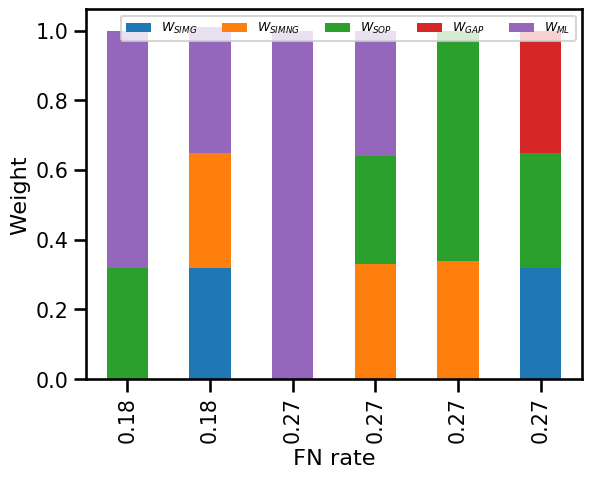
\includegraphics[width=0.22\textwidth]{weight-A/BB11018-good-weight}}
		\subfloat[BB11007]{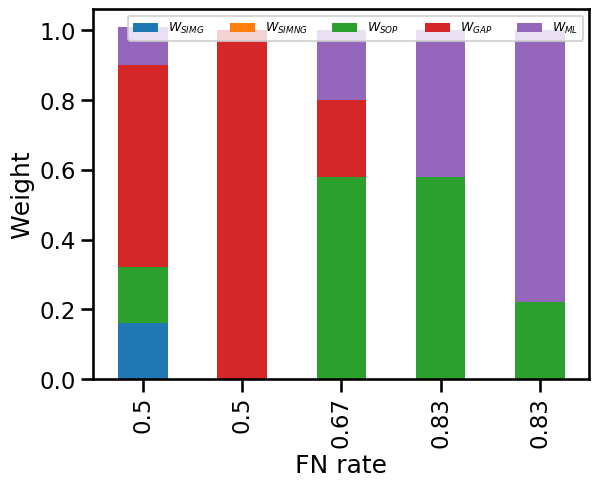
\includegraphics[width=0.25\textwidth]{weight-B-ml/BB11007-good-weight}}
		\subfloat[BB20012]{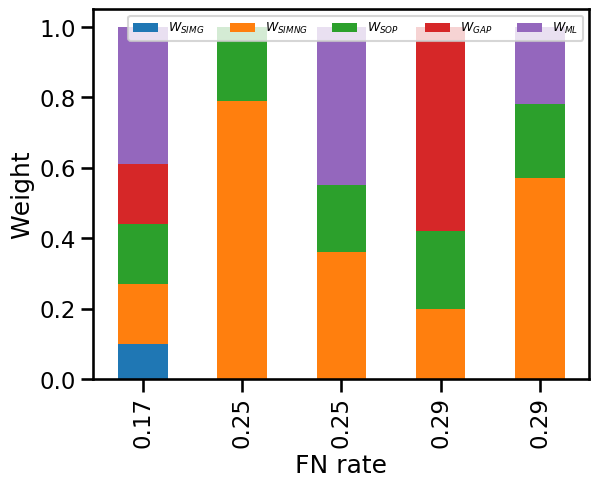
\includegraphics[width=0.25\textwidth]{weight-B-ml/BB20012-good-weight}}\\
		\subfloat[BB30026]{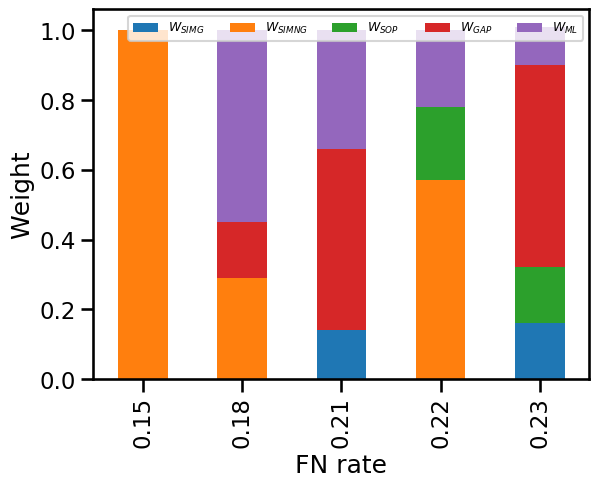
\includegraphics[width=0.25\textwidth]{weight-B-ml/BB30026-good-weight}}%
		\subfloat[BB50009]{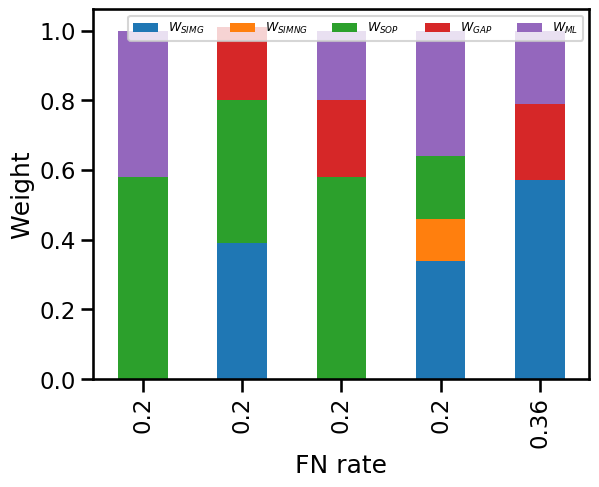
\includegraphics[width=0.25\textwidth]{weight-B-ml/BB50009-good-weight}}%
	\end{adjustwidth}
	\caption{Visualization of five input weight vectors detected by our supervised regression based pipeline on four arbitrary datasets in set B. The y-axis portrays the weight values and the x-axis marks the achieved FN rate. The weight vectors are sorted in ascending order based on the achieved FN rate. }
	\label{fig:some-good-weight-ml}
\end{figure}

\begin{table}[!htbp]
	\small
	\caption{PMAO variants based on selection of five input weight vectors.}
	\begin{tabular}{l|L{7cm}}
		Variant &  How to select the five input weight vectors for PMAO\\
		\hline
		PMAO-5DW  &  Detected from 100 well-spaced vectors based on lower FN rates predicted by a XGBoost regressor\\
		\hline
		PMAO-5RW  &  Randomly sampled from 30 well-spaced weight vectors \\
	\end{tabular}%
	\label{tab:variants-weight}%
\end{table}%


% Table generated by Excel2LaTeX from sheet 'stat-8I-30w-ML-w'
\begin{table}[!htbp]
	\small
	\caption{Comparison of the five solutions generated by two PMAO variants with respect to PASTA based on FN rate on datasets under set B. For PMAO, we show the best and average FN rate of the five solutions. The better values are marked with darker shade.}
	\begin{tabular}{|l|r|r|r|r|r|}
		\hline
		\multirow{2}{*}{Dataset} & \multirow{2}{*}{\makecell{PASTA\\FN rate}} & \multicolumn{2}{c|}{\makecell{PMO-5DW\\FN rate}} & \multicolumn{2}{c|}{\makecell{PMO-5RW\\FN rate}} \\
		\cline{3-6}          &       & Best & Avg & Best & Avg \\
		\hline
		BB11007 & \cellcolor[rgb]{ .686,  .871,  .733}0.50 & \cellcolor[rgb]{ .686,  .871,  .733}0.50 & \cellcolor[rgb]{ .988,  1,  .992}0.67 & \cellcolor[rgb]{ .384,  .745,  .478}0.33 & \cellcolor[rgb]{ .804,  .922,  .835}0.57 \\
		\hline
		BB11034 & \cellcolor[rgb]{ .635,  .851,  .69}0.40 & \cellcolor[rgb]{ .384,  .745,  .478}0.20 & \cellcolor[rgb]{ .584,  .827,  .647}0.36 & \cellcolor[rgb]{ .384,  .745,  .478}0.20 & \cellcolor[rgb]{ .988,  1,  .992}0.68 \\
		\hline
		BB11038 & \cellcolor[rgb]{ .384,  .745,  .478}0.40 & \cellcolor[rgb]{ .384,  .745,  .478}0.40 & \cellcolor[rgb]{ .988,  1,  .992}0.64 & \cellcolor[rgb]{ .384,  .745,  .478}0.40 & \cellcolor[rgb]{ .686,  .871,  .733}0.52 \\
		\hline
		BB11019 & \cellcolor[rgb]{ .384,  .745,  .478}0.29 & \cellcolor[rgb]{ .384,  .745,  .478}0.29 & \cellcolor[rgb]{ .384,  .745,  .478}0.29 & \cellcolor[rgb]{ .384,  .745,  .478}0.29 & \cellcolor[rgb]{ .988,  1,  .992}0.31 \\
		\hline
		BB12005 & \cellcolor[rgb]{ .384,  .745,  .478}0.33 & \cellcolor[rgb]{ .384,  .745,  .478}0.33 & \cellcolor[rgb]{ .988,  1,  .992}0.37 & \cellcolor[rgb]{ .384,  .745,  .478}0.33 & \cellcolor[rgb]{ .988,  1,  .992}0.37 \\
		\hline
		BB12029 & \cellcolor[rgb]{ .988,  1,  .992}0.44 & \cellcolor[rgb]{ .384,  .745,  .478}0.33 & \cellcolor[rgb]{ .745,  .894,  .784}0.40 & \cellcolor[rgb]{ .988,  1,  .992}0.44 & \cellcolor[rgb]{ .988,  1,  .992}0.44 \\
		\hline
		BB12026 & \cellcolor[rgb]{ .682,  .871,  .733}0.53 & \cellcolor[rgb]{ .384,  .745,  .478}0.47 & \cellcolor[rgb]{ .682,  .871,  .733}0.53 & \cellcolor[rgb]{ .682,  .871,  .733}0.53 & \cellcolor[rgb]{ .988,  1,  .992}0.60 \\
		\hline
		BB12037 & \cellcolor[rgb]{ .384,  .745,  .478}0.40 & \cellcolor[rgb]{ .914,  .969,  .929}0.70 & \cellcolor[rgb]{ .988,  1,  .992}0.74 & \cellcolor[rgb]{ .384,  .745,  .478}0.40 & \cellcolor[rgb]{ .737,  .894,  .78}0.60 \\
		\hline
		BB20002 & \cellcolor[rgb]{ .549,  .816,  .62}0.65 & \cellcolor[rgb]{ .384,  .745,  .478}0.59 & \cellcolor[rgb]{ .651,  .855,  .706}0.68 & \cellcolor[rgb]{ .384,  .745,  .478}0.59 & \cellcolor[rgb]{ .988,  1,  .992}0.80 \\
		\hline
		BB20012 & \cellcolor[rgb]{ .988,  1,  .992}0.29 & \cellcolor[rgb]{ .384,  .745,  .478}0.17 & \cellcolor[rgb]{ .784,  .914,  .82}0.25 & \cellcolor[rgb]{ .584,  .827,  .647}0.21 & \cellcolor[rgb]{ .824,  .929,  .855}0.26 \\
		\hline
		BB20030 & \cellcolor[rgb]{ .384,  .745,  .478}0.64 & \cellcolor[rgb]{ .384,  .745,  .478}0.64 & \cellcolor[rgb]{ .988,  1,  .992}0.69 & \cellcolor[rgb]{ .384,  .745,  .478}0.64 & \cellcolor[rgb]{ .933,  .976,  .945}0.68 \\
		\hline
		BB20037 & \cellcolor[rgb]{ .384,  .745,  .478}0.13 & \cellcolor[rgb]{ .549,  .816,  .62}0.16 & \cellcolor[rgb]{ .8,  .922,  .831}0.21 & \cellcolor[rgb]{ .886,  .957,  .906}0.23 & \cellcolor[rgb]{ .988,  1,  .992}0.25 \\
		\hline
		BB30003 & \cellcolor[rgb]{ .988,  1,  .992}0.30 & \cellcolor[rgb]{ .384,  .745,  .478}0.28 & \cellcolor[rgb]{ .706,  .878,  .749}0.29 & \cellcolor[rgb]{ .584,  .827,  .647}0.29 & \cellcolor[rgb]{ .945,  .98,  .957}0.30 \\
		\hline
		BB30021 & \cellcolor[rgb]{ .941,  .98,  .953}0.36 & \cellcolor[rgb]{ .384,  .745,  .478}0.32 & \cellcolor[rgb]{ .988,  1,  .992}0.36 & \cellcolor[rgb]{ .384,  .745,  .478}0.32 & \cellcolor[rgb]{ .784,  .914,  .82}0.35 \\
		\hline
		BB30026 & \cellcolor[rgb]{ .859,  .945,  .882}0.19 & \cellcolor[rgb]{ .384,  .745,  .478}0.15 & \cellcolor[rgb]{ .922,  .973,  .937}0.20 & \cellcolor[rgb]{ .702,  .878,  .745}0.18 & \cellcolor[rgb]{ .988,  1,  .992}0.20 \\
		\hline
		BB30011 & \cellcolor[rgb]{ .988,  1,  .992}0.35 & \cellcolor[rgb]{ .384,  .745,  .478}0.32 & \cellcolor[rgb]{ .804,  .922,  .835}0.35 & \cellcolor[rgb]{ .988,  1,  .992}0.35 & \cellcolor[rgb]{ .988,  1,  .992}0.35 \\
		\hline
		BB40009 & \cellcolor[rgb]{ .384,  .745,  .478}0.19 & \cellcolor[rgb]{ .384,  .745,  .478}0.19 & \cellcolor[rgb]{ .533,  .808,  .604}0.20 & \cellcolor[rgb]{ .384,  .745,  .478}0.19 & \cellcolor[rgb]{ .988,  1,  .992}0.24 \\
		\hline
		BB40019 & \cellcolor[rgb]{ .988,  1,  .992}0.43 & \cellcolor[rgb]{ .384,  .745,  .478}0.29 & \cellcolor[rgb]{ .745,  .898,  .784}0.37 & \cellcolor[rgb]{ .384,  .745,  .478}0.29 & \cellcolor[rgb]{ .624,  .847,  .682}0.34 \\
		\hline
		BB40033 & \cellcolor[rgb]{ .988,  1,  .992}0.13 & \cellcolor[rgb]{ .384,  .745,  .478}0.06 & \cellcolor[rgb]{ .867,  .949,  .886}0.11 & \cellcolor[rgb]{ .384,  .745,  .478}0.06 & \cellcolor[rgb]{ .867,  .949,  .886}0.11 \\
		\hline
		BB40006 & \cellcolor[rgb]{ .384,  .745,  .478}0.00 & \cellcolor[rgb]{ .384,  .745,  .478}0.00 & \cellcolor[rgb]{ .886,  .957,  .906}0.09 & \cellcolor[rgb]{ .886,  .957,  .906}0.09 & \cellcolor[rgb]{ .988,  1,  .992}0.11 \\
		\hline
		BB50002 & \cellcolor[rgb]{ .718,  .886,  .761}0.50 & \cellcolor[rgb]{ .384,  .745,  .478}0.40 & \cellcolor[rgb]{ .851,  .941,  .875}0.54 & \cellcolor[rgb]{ .718,  .886,  .761}0.50 & \cellcolor[rgb]{ .988,  1,  .992}0.58 \\
		\hline
		BB50009 & \cellcolor[rgb]{ .988,  1,  .992}0.24 & \cellcolor[rgb]{ .835,  .933,  .863}0.20 & \cellcolor[rgb]{ .957,  .984,  .965}0.23 & \cellcolor[rgb]{ .384,  .745,  .478}0.08 & \cellcolor[rgb]{ .835,  .933,  .863}0.20 \\
		\hline
		BB50014 & \cellcolor[rgb]{ .384,  .745,  .478}0.41 & \cellcolor[rgb]{ .384,  .745,  .478}0.41 & \cellcolor[rgb]{ .867,  .949,  .886}0.44 & \cellcolor[rgb]{ .988,  1,  .992}0.44 & \cellcolor[rgb]{ .988,  1,  .992}0.44 \\
		\hline
		BB50006 & \cellcolor[rgb]{ .749,  .898,  .788}0.21 & \cellcolor[rgb]{ .384,  .745,  .478}0.14 & \cellcolor[rgb]{ .839,  .937,  .867}0.23 & \cellcolor[rgb]{ .655,  .859,  .71}0.19 & \cellcolor[rgb]{ .988,  1,  .992}0.26 \\
		\hline
	\end{tabular}%
	\label{tab:pmao-5pw-b}%
\end{table}%

% Table generated by Excel2LaTeX from sheet 'stat test'
\begin{table}[!htbp]
	\small
	\caption{\underline{Friedman Aligned Ranks test (Column 2):} Friedman Aligned ranks (lower is better) of PASTA and the two PMAO variants based on the best FN rates reported in Table~\ref{tab:pmao-5pw-b}. We also show the computed statistics and corresponding $ p $-value. 
	\underline{Holm's post-hoc procedure (Columns 3 - 5):} Comparison among PASTA and two PMAO variants using the Holm's post-hoc procedures. Each entry shows the adjusted $p$-value which indicates the significance of the difference in performance between two methods.}
	\begin{adjustwidth}{-0.7cm}{}
	\begin{tabular}{|l|r||ccc|}
		\hline
		\multicolumn{1}{|c|}{1} & \multicolumn{1}{c||}{2} & \multicolumn{1}{c|}{3} & \multicolumn{1}{c|}{4} & 5 \\
		\hline
		\multirow{2}{*}{\makecell{Method}} & \multirow{2}{*}{\makecell{Friedman\\Aligned Rank*}} & \multicolumn{3}{c|}{Holm's adjusted $p$-value} \\
		\cline{3-5}          &       & \multicolumn{1}{l|}{PMAO-5DW} & \multicolumn{1}{l|}{PMAO-5RW} & \multicolumn{1}{l|}{PASTA} \\
		\hline
		PMAO-5DW & 27.0000 & \multicolumn{1}{c|}{-} & \multicolumn{1}{r|}{0.1972} & \multicolumn{1}{r|}{\cellcolor[rgb]{ .384,  .745,  .478}0.0018} \\
		\hline
		PMAO-5RW & 34.7917 & \multicolumn{1}{r|}{0.1972} & \multicolumn{1}{c|}{-} & \multicolumn{1}{r|}{0.0650} \\
		\hline
		PASTA & 47.7083 & \multicolumn{1}{r|}{\cellcolor[rgb]{ .384,  .745,  .478}0.0018} & \multicolumn{1}{r|}{0.0650} & - \\
		\hline
		*Statistic & 8.5117 & \multicolumn{3}{c|}{\multirow{2}{*}{N/A}} \\
		\cline{1-2}    *$p$-value & 0.0142 & \multicolumn{3}{c|}{} \\
		\hline
	\end{tabular}%
	\label{tab:test-ml-weights}%
	\end{adjustwidth}
\end{table}%

\subsubsection{Obtain one solution from PMAO-5DW}
In pursuit of a single high-quality solution, we proceed even further. We employ the following two schemes to obtain a single high-quality solution by summarizing the five solutions generated by PMAO-5DW.
\begin{enumerate}
	%\item NSUM: Select the solution whose sum of normalized (min-max) objective values is the maximum among the 30 candidates
	\item GRED: Summarize the five candidate trees using greedy consensus method of PAUP* (Phylogenetic Analysis Using PAUP)\footnote{https://paup.phylosolutions.com/}.
	\item AST: Summarize the five candidate trees based on quartet consistency using ASTRAL~\cite{zhang2018astral}, one of the most accurate and widely used coalescent-based methods to infer species trees.
\end{enumerate}
We compare the FN rates of the aforementioned summarizing schemes with PASTA on all BAliBASE 3.0 datasets, except set A to eliminate any bias due to their involvement in training the regression model, in Supplementary Table~\ref{tab:obtain-single-ml}. Then we apply the Friedman Aligned Ranks test followed by Holm's post-hoc procedure on these data and report the results in Table~\ref{tab:test-summary}. We observe that GRED and AST schemes exhibit significantly better performance than PASTA, with GRED being the top performer. However, these schemes are not always able to obtain the best FN rates of PMAO-5DW, and thus we see that PASTA performs better than GRED and AST (Supplementary Table~\ref{tab:obtain-single-ml}) in 37 cases out of 191. This suggests that, although promising, further refinement of this approach or application of other strategies may be in order.

% Table generated by Excel2LaTeX from sheet 'stat test'
\begin{table}[htbp]
  \small
  \caption{\underline{Friedman Aligned Ranks test (Column 2):} Friedman Aligned ranks (lower is better) of PASTA and two schemes for summarizing five solutions generated by PMAO-5DW based on FN rates reported in Supplementary Table~\ref{tab:obtain-single-ml}. We also show the computed statistics and corresponding $ p $-value. 
	\underline{Holm's post-hoc procedure (Columns 3 - 5):} Comparison among PASTA and two summarizing schemes using the Holm's post-hoc procedures. Each entry shows the adjusted $p$-value which indicates the significance of the difference in performance between two methods.}
    \begin{tabular}{|l|r|ccc|}
    \hline
    \multicolumn{1}{|c|}{1} & \multicolumn{1}{c|}{2} & \multicolumn{1}{c|}{3} & \multicolumn{1}{c|}{4} & 5 \\
    \hline
	\multirow{2}{*}{\makecell{Methods}} & \multirow{2}{*}{\makecell{Friedman\\Aligned rank*}} & \multicolumn{3}{c|}{Holm's adjusted $p$-value} \\
\cline{3-5}          &       & \multicolumn{1}{l|}{GRED} & \multicolumn{1}{l|}{AST} & \multicolumn{1}{l|}{PASTA} \\
    \hline
    GRED  & 263.9922 & \multicolumn{1}{c|}{-} & \multicolumn{1}{r|}{0.5982} & \multicolumn{1}{r|}{\cellcolor[rgb]{ 0,  .69,  .314}0.0012} \\
    \hline
    AST   & 272.9189 & \multicolumn{1}{r|}{0.5982} & \multicolumn{1}{c|}{-} & \multicolumn{1}{r|}{\cellcolor[rgb]{ 0,  .69,  .314}0.0051} \\
    \hline
    PASTA & 324.0890 & \multicolumn{1}{r|}{\cellcolor[rgb]{ 0,  .69,  .314}0.0012} & \multicolumn{1}{r|}{\cellcolor[rgb]{ 0,  .69,  .314}0.0051} & - \\
    \hline
    *Statistic & 10.7149 & \multicolumn{3}{c|}{\multirow{2}{*}{N/A}} \\
\cline{1-2}    *$p$-value & 0.0047 & \multicolumn{3}{c|}{} \\
    \hline
    \end{tabular}%
  \label{tab:test-summary}%
\end{table}%















\begin{comment}
% \begin{table}[!htbp]
% 	\small
% 	\caption{PMAO variants based on iteration count and guide tree decomposition strategy. }
% 	\begin{tabular}{l|r|l}
% 		Variant & Iteration & Tree decomposition\\
% 		\hline
% 		PMAO-3I-D  & 3     & Default (\textit{mincluster}) \\
% 		\hline
% 		PMAO-8I-D  & 8     & Default (\textit{mincluster}) \\
% 		\hline
% 		PMAO-3I-S  & 3     & Stochastic \\
% 		\hline
% 		PMAO-8I-S  & 8     & Stochastic\\
% 	\end{tabular}%
% 	\label{tab:variants}%
% \end{table}%
% Table generated by Excel2LaTeX from sheet 'Sheet7 (2)'
\begin{table}[!htbp]
	\small
	\caption{Comparison of the three selection schemes used to obtain a single solution from the 30 solutions generated by PMAO on datasets under set A in terms of FN rate. We also include PASTA's FN rate and PMAO best FN rate. The better values are marked with darker shade.}
	\begin{tabular}{|l|r|r|r|r|r|}
		\hline
		\multirow{2}{*}{Dataset} & \multirow{2}{*}{PASTA} & \multicolumn{3}{c|}{Selection scheme} & \multirow{2}{*}{\makecell{PMAO\\Best}} \\
		\cline{3-5}          &       & \multicolumn{1}{l|}{NSUM} & \multicolumn{1}{l|}{GRED} & \multicolumn{1}{l|}{AST} &  \\
		\hline
		BB11005 & \cellcolor[rgb]{ .988,  1,  .992}0.55 & \cellcolor[rgb]{ .431,  .824,  .51}0.27 & \cellcolor[rgb]{ .431,  .824,  .51}0.27 & \cellcolor[rgb]{ .431,  .824,  .51}0.27 & \cellcolor[rgb]{ .384,  .725,  .478}0.09 \\
		\hline
		BB11018 & \cellcolor[rgb]{ .988,  1,  .992}0.27 & \cellcolor[rgb]{ .988,  1,  .992}0.27 & \cellcolor[rgb]{ .988,  1,  .992}0.27 & \cellcolor[rgb]{ .988,  1,  .992}0.27 & \cellcolor[rgb]{ .384,  .725,  .478}0.18 \\
		\hline
		BB11033 & \cellcolor[rgb]{ .384,  .725,  .478}0.38 & \cellcolor[rgb]{ .988,  1,  .992}0.50 & \cellcolor[rgb]{ .988,  1,  .992}0.50 & \cellcolor[rgb]{ .988,  1,  .992}0.50 & \cellcolor[rgb]{ .384,  .725,  .478}0.38 \\
		\hline
		BB11020 & \cellcolor[rgb]{ .988,  1,  .992}0.83 & \cellcolor[rgb]{ .431,  .824,  .51}0.67 & \cellcolor[rgb]{ .431,  .824,  .51}0.67 & \cellcolor[rgb]{ .431,  .824,  .51}0.67 & \cellcolor[rgb]{ .384,  .725,  .478}0.33 \\
		\hline
		BB12001 & \cellcolor[rgb]{ .431,  .824,  .51}0.25 & \cellcolor[rgb]{ .384,  .725,  .478}0.13 & \cellcolor[rgb]{ .988,  1,  .992}0.38 & \cellcolor[rgb]{ .988,  1,  .992}0.38 & \cellcolor[rgb]{ .384,  .725,  .478}0.13 \\
		\hline
		BB12013 & \cellcolor[rgb]{ .988,  1,  .992}0.20 & \cellcolor[rgb]{ .988,  1,  .992}0.20 & \cellcolor[rgb]{ .988,  1,  .992}0.20 & \cellcolor[rgb]{ .988,  1,  .992}0.20 & \cellcolor[rgb]{ .988,  1,  .992}0.20 \\
		\hline
		BB12022 & \cellcolor[rgb]{ .988,  1,  .992}0.00 & \cellcolor[rgb]{ .988,  1,  .992}0.00 & \cellcolor[rgb]{ .988,  1,  .992}0.00 & \cellcolor[rgb]{ .988,  1,  .992}0.00 & \cellcolor[rgb]{ .988,  1,  .992}0.00 \\
		\hline
		BB12035 & \cellcolor[rgb]{ .384,  .725,  .478}0.00 & \cellcolor[rgb]{ .988,  1,  .992}0.46 & \cellcolor[rgb]{ .431,  .824,  .51}0.04 & \cellcolor[rgb]{ .431,  .824,  .51}0.04 & \cellcolor[rgb]{ .431,  .824,  .51}0.04 \\
		\hline
		BB12044 & \cellcolor[rgb]{ .988,  1,  .992}0.50 & \cellcolor[rgb]{ .988,  1,  .992}0.50 & \cellcolor[rgb]{ .988,  1,  .992}0.50 & \cellcolor[rgb]{ .988,  1,  .992}0.50 & \cellcolor[rgb]{ .384,  .725,  .478}0.38 \\
		\hline
		BB20001 & \cellcolor[rgb]{ .988,  1,  .992}0.54 & \cellcolor[rgb]{ .431,  .824,  .51}0.46 & \cellcolor[rgb]{ .431,  .824,  .51}0.46 & \cellcolor[rgb]{ .431,  .824,  .51}0.46 & \cellcolor[rgb]{ .384,  .725,  .478}0.23 \\
		\hline
		BB20010 & \cellcolor[rgb]{ .431,  .824,  .51}0.35 & \cellcolor[rgb]{ .424,  .808,  .502}0.31 & \cellcolor[rgb]{ .988,  1,  .992}0.38 & \cellcolor[rgb]{ .431,  .824,  .51}0.35 & \cellcolor[rgb]{ .384,  .725,  .478}0.08 \\
		\hline
		BB20022 & \cellcolor[rgb]{ .431,  .824,  .51}0.11 & \cellcolor[rgb]{ .984,  .996,  .988}0.13 & \cellcolor[rgb]{ .988,  1,  .992}0.13 & \cellcolor[rgb]{ .431,  .824,  .51}0.11 & \cellcolor[rgb]{ .384,  .725,  .478}0.09 \\
		\hline
		BB20033 & \cellcolor[rgb]{ .431,  .824,  .51}0.36 & \cellcolor[rgb]{ .384,  .725,  .478}0.24 & \cellcolor[rgb]{ .988,  1,  .992}0.38 & \cellcolor[rgb]{ .988,  1,  .992}0.38 & \cellcolor[rgb]{ .384,  .725,  .478}0.24 \\
		\hline
		BB20041 & \cellcolor[rgb]{ .431,  .824,  .51}0.38 & \cellcolor[rgb]{ .988,  1,  .992}0.44 & \cellcolor[rgb]{ .431,  .824,  .51}0.38 & \cellcolor[rgb]{ .408,  .773,  .494}0.36 & \cellcolor[rgb]{ .384,  .725,  .478}0.33 \\
		\hline
		BB30002 & \cellcolor[rgb]{ .431,  .824,  .51}0.32 & \cellcolor[rgb]{ .988,  1,  .992}0.36 & \cellcolor[rgb]{ .988,  1,  .992}0.36 & \cellcolor[rgb]{ .431,  .824,  .51}0.32 & \cellcolor[rgb]{ .384,  .725,  .478}0.18 \\
		\hline
		BB30008 & \cellcolor[rgb]{ .427,  .82,  .506}0.33 & \cellcolor[rgb]{ .988,  1,  .992}0.45 & \cellcolor[rgb]{ .569,  .867,  .627}0.36 & \cellcolor[rgb]{ .431,  .824,  .51}0.33 & \cellcolor[rgb]{ .384,  .725,  .478}0.21 \\
		\hline
		BB30015 & \cellcolor[rgb]{ .988,  1,  .992}0.17 & \cellcolor[rgb]{ .988,  1,  .992}0.17 & \cellcolor[rgb]{ .988,  1,  .992}0.17 & \cellcolor[rgb]{ .988,  1,  .992}0.17 & \cellcolor[rgb]{ .988,  1,  .992}0.17 \\
		\hline
		BB30022 & \cellcolor[rgb]{ .988,  1,  .992}0.51 & \cellcolor[rgb]{ .412,  .788,  .498}0.49 & \cellcolor[rgb]{ .988,  1,  .992}0.51 & \cellcolor[rgb]{ .988,  1,  .992}0.51 & \cellcolor[rgb]{ .384,  .725,  .478}0.46 \\
		\hline
		BB40001 & \cellcolor[rgb]{ .431,  .824,  .51}0.48 & \cellcolor[rgb]{ .431,  .824,  .51}0.48 & \cellcolor[rgb]{ .988,  1,  .992}0.52 & \cellcolor[rgb]{ .988,  1,  .992}0.52 & \cellcolor[rgb]{ .384,  .725,  .478}0.36 \\
		\hline
		BB40013 & \cellcolor[rgb]{ .616,  .878,  .667}0.38 & \cellcolor[rgb]{ .988,  1,  .992}0.44 & \cellcolor[rgb]{ .431,  .824,  .51}0.34 & \cellcolor[rgb]{ .416,  .788,  .498}0.31 & \cellcolor[rgb]{ .384,  .725,  .478}0.25 \\
		\hline
		BB40025 & \cellcolor[rgb]{ .988,  1,  .992}0.00 & \cellcolor[rgb]{ .988,  1,  .992}0.00 & \cellcolor[rgb]{ .988,  1,  .992}0.00 & \cellcolor[rgb]{ .988,  1,  .992}0.00 & \cellcolor[rgb]{ .988,  1,  .992}0.00 \\
		\hline
		BB40038 & \cellcolor[rgb]{ .988,  1,  .992}0.25 & \cellcolor[rgb]{ .416,  .788,  .498}0.20 & \cellcolor[rgb]{ .988,  1,  .992}0.25 & \cellcolor[rgb]{ .988,  1,  .992}0.25 & \cellcolor[rgb]{ .384,  .725,  .478}0.10 \\
		\hline
		BB40048 & \cellcolor[rgb]{ .988,  1,  .992}0.43 & \cellcolor[rgb]{ .384,  .725,  .478}0.29 & \cellcolor[rgb]{ .384,  .725,  .478}0.29 & \cellcolor[rgb]{ .384,  .725,  .478}0.29 & \cellcolor[rgb]{ .384,  .725,  .478}0.29 \\
		\hline
		BB50001 & \cellcolor[rgb]{ .384,  .725,  .478}0.29 & \cellcolor[rgb]{ .988,  1,  .992}0.32 & \cellcolor[rgb]{ .384,  .725,  .478}0.29 & \cellcolor[rgb]{ .384,  .725,  .478}0.29 & \cellcolor[rgb]{ .384,  .725,  .478}0.29 \\
		\hline
		BB50005 & \cellcolor[rgb]{ .988,  1,  .992}0.38 & \cellcolor[rgb]{ .988,  1,  .992}0.38 & \cellcolor[rgb]{ .988,  1,  .992}0.38 & \cellcolor[rgb]{ .988,  1,  .992}0.38 & \cellcolor[rgb]{ .384,  .725,  .478}0.25 \\
		\hline
		BB50010 & \cellcolor[rgb]{ .384,  .725,  .478}0.00 & \cellcolor[rgb]{ .988,  1,  .992}0.14 & \cellcolor[rgb]{ .988,  1,  .992}0.14 & \cellcolor[rgb]{ .988,  1,  .992}0.14 & \cellcolor[rgb]{ .384,  .725,  .478}0.00 \\
		\hline
		BB50016 & \cellcolor[rgb]{ .988,  1,  .992}0.47 & \cellcolor[rgb]{ .431,  .824,  .51}0.13 & \cellcolor[rgb]{ .431,  .824,  .51}0.13 & \cellcolor[rgb]{ .431,  .824,  .51}0.13 & \cellcolor[rgb]{ .384,  .725,  .478}0.07 \\
		\hline
	\end{tabular}%
	\label{tab:select-one-a}%
\end{table}%


% Table generated by Excel2LaTeX from sheet 'Sheet7 (2)'
\begin{table}[!htbp]
	\small
	\caption{Comparison of the three selection schemes used to obtain a single solution from the 30 solutions generated by PMAO on datasets under set A in terms of FN rate. We also include PASTA's FN rate and PMAO best FN rate. The better values are marked with darker shade.}
	\begin{tabular}{|l|r|r|r|r|r|}
		\hline
		\multirow{2}{*}{Dataset} & \multirow{2}{*}{PASTA} & \multicolumn{3}{c|}{Selection scheme} & \multirow{2}{*}{\makecell{PMAO\\Best}} \\
		\cline{3-5}          &       & \multicolumn{1}{l|}{NSUM} & \multicolumn{1}{l|}{GRED} & \multicolumn{1}{l|}{AST} &  \\
		\hline
		BB11007 & \cellcolor[rgb]{ .408,  .773,  .494}0.50 & \cellcolor[rgb]{ .988,  1,  .992}0.83 & \cellcolor[rgb]{ .431,  .824,  .51}0.67 & \cellcolor[rgb]{ .431,  .824,  .51}0.67 & \cellcolor[rgb]{ .384,  .725,  .478}0.33 \\
		\hline
		BB11034 & \cellcolor[rgb]{ .431,  .824,  .51}0.40 & \cellcolor[rgb]{ .988,  1,  .992}1.00 & \cellcolor[rgb]{ .431,  .824,  .51}0.40 & \cellcolor[rgb]{ .431,  .824,  .51}0.40 & \cellcolor[rgb]{ .384,  .725,  .478}0.20 \\
		\hline
		BB11038 & \cellcolor[rgb]{ .988,  1,  .992}0.40 & \cellcolor[rgb]{ .988,  1,  .992}0.40 & \cellcolor[rgb]{ .988,  1,  .992}0.40 & \cellcolor[rgb]{ .988,  1,  .992}0.40 & \cellcolor[rgb]{ .384,  .725,  .478}0.00 \\
		\hline
		BB11019 & \cellcolor[rgb]{ .988,  1,  .992}0.29 & \cellcolor[rgb]{ .988,  1,  .992}0.29 & \cellcolor[rgb]{ .988,  1,  .992}0.29 & \cellcolor[rgb]{ .988,  1,  .992}0.29 & \cellcolor[rgb]{ .384,  .725,  .478}0.14 \\
		\hline
		BB12005 & \cellcolor[rgb]{ .384,  .725,  .478}0.33 & \cellcolor[rgb]{ .384,  .725,  .478}0.33 & \cellcolor[rgb]{ .988,  1,  .992}0.33 & \cellcolor[rgb]{ .988,  1,  .992}0.33 & \cellcolor[rgb]{ .384,  .725,  .478}0.33 \\
		\hline
		BB12029 & \cellcolor[rgb]{ .988,  1,  .992}0.44 & \cellcolor[rgb]{ .988,  1,  .992}0.44 & \cellcolor[rgb]{ .988,  1,  .992}0.44 & \cellcolor[rgb]{ .988,  1,  .992}0.44 & \cellcolor[rgb]{ .384,  .725,  .478}0.33 \\
		\hline
		BB12026 & \cellcolor[rgb]{ .706,  .91,  .749}0.53 & \cellcolor[rgb]{ .988,  1,  .992}0.60 & \cellcolor[rgb]{ .431,  .824,  .51}0.47 & \cellcolor[rgb]{ .431,  .824,  .51}0.47 & \cellcolor[rgb]{ .384,  .725,  .478}0.33 \\
		\hline
		BB12037 & \cellcolor[rgb]{ .431,  .824,  .51}0.40 & \cellcolor[rgb]{ .431,  .824,  .51}0.40 & \cellcolor[rgb]{ .988,  1,  .992}0.60 & \cellcolor[rgb]{ .431,  .824,  .51}0.40 & \cellcolor[rgb]{ .384,  .725,  .478}0.10 \\
		\hline
		BB20002 & \cellcolor[rgb]{ .431,  .824,  .51}0.65 & \cellcolor[rgb]{ .988,  1,  .992}0.76 & \cellcolor[rgb]{ .431,  .824,  .51}0.65 & \cellcolor[rgb]{ .431,  .824,  .51}0.65 & \cellcolor[rgb]{ .384,  .725,  .478}0.53 \\
		\hline
		BB20012 & \cellcolor[rgb]{ .8,  .941,  .831}0.29 & \cellcolor[rgb]{ .988,  1,  .992}0.33 & \cellcolor[rgb]{ .431,  .824,  .51}0.21 & \cellcolor[rgb]{ .431,  .824,  .51}0.21 & \cellcolor[rgb]{ .384,  .725,  .478}0.08 \\
		\hline
		BB20030 & \cellcolor[rgb]{ .384,  .725,  .478}0.64 & \cellcolor[rgb]{ .384,  .725,  .478}0.64 & \cellcolor[rgb]{ .988,  1,  .992}0.70 & \cellcolor[rgb]{ .988,  1,  .992}0.70 & \cellcolor[rgb]{ .384,  .725,  .478}0.64 \\
		\hline
		BB20037 & \cellcolor[rgb]{ .384,  .725,  .478}0.13 & \cellcolor[rgb]{ .988,  1,  .992}0.27 & \cellcolor[rgb]{ .431,  .824,  .51}0.23 & \cellcolor[rgb]{ .431,  .824,  .51}0.23 & \cellcolor[rgb]{ .384,  .725,  .478}0.13 \\
		\hline
		BB30003 & \cellcolor[rgb]{ .8,  .937,  .827}0.30 & \cellcolor[rgb]{ .988,  1,  .992}0.31 & \cellcolor[rgb]{ .431,  .824,  .51}0.29 & \cellcolor[rgb]{ .431,  .824,  .51}0.29 & \cellcolor[rgb]{ .384,  .725,  .478}0.26 \\
		\hline
		BB30021 & \cellcolor[rgb]{ .416,  .792,  .498}0.36 & \cellcolor[rgb]{ .988,  1,  .992}0.39 & \cellcolor[rgb]{ .431,  .824,  .51}0.37 & \cellcolor[rgb]{ .431,  .824,  .51}0.37 & \cellcolor[rgb]{ .384,  .725,  .478}0.32 \\
		\hline
		BB30026 & \cellcolor[rgb]{ .42,  .796,  .502}0.19 & \cellcolor[rgb]{ .431,  .824,  .51}0.21 & \cellcolor[rgb]{ .988,  1,  .992}0.22 & \cellcolor[rgb]{ .988,  1,  .992}0.22 & \cellcolor[rgb]{ .384,  .725,  .478}0.15 \\
		\hline
		BB30011 & \cellcolor[rgb]{ .988,  1,  .992}0.35 & \cellcolor[rgb]{ .988,  1,  .992}0.35 & \cellcolor[rgb]{ .431,  .824,  .51}0.34 & \cellcolor[rgb]{ .431,  .824,  .51}0.34 & \cellcolor[rgb]{ .384,  .725,  .478}0.31 \\
		\hline
		BB40009 & \cellcolor[rgb]{ .988,  1,  .992}0.19 & \cellcolor[rgb]{ .988,  1,  .992}0.19 & \cellcolor[rgb]{ .384,  .725,  .478}0.13 & \cellcolor[rgb]{ .384,  .725,  .478}0.13 & \cellcolor[rgb]{ .384,  .725,  .478}0.13 \\
		\hline
		BB40019 & \cellcolor[rgb]{ .988,  1,  .992}0.43 & \cellcolor[rgb]{ .384,  .725,  .478}0.29 & \cellcolor[rgb]{ .988,  1,  .992}0.43 & \cellcolor[rgb]{ .988,  1,  .992}0.43 & \cellcolor[rgb]{ .384,  .725,  .478}0.29 \\
		\hline
		BB40033 & \cellcolor[rgb]{ .988,  1,  .992}0.13 & \cellcolor[rgb]{ .988,  1,  .992}0.13 & \cellcolor[rgb]{ .988,  1,  .992}0.13 & \cellcolor[rgb]{ .384,  .725,  .478}0.06 & \cellcolor[rgb]{ .384,  .725,  .478}0.06 \\
		\hline
		BB40006 & \cellcolor[rgb]{ .384,  .725,  .478}0.00 & \cellcolor[rgb]{ .384,  .725,  .478}0.00 & \cellcolor[rgb]{ .384,  .725,  .478}0.00 & \cellcolor[rgb]{ .988,  1,  .992}0.09 & \cellcolor[rgb]{ .384,  .725,  .478}0.00 \\
		\hline
		BB50002 & \cellcolor[rgb]{ .988,  1,  .992}0.50 & \cellcolor[rgb]{ .988,  1,  .992}0.50 & \cellcolor[rgb]{ .988,  1,  .992}0.50 & \cellcolor[rgb]{ .988,  1,  .992}0.50 & \cellcolor[rgb]{ .384,  .725,  .478}0.40 \\
		\hline
		BB50009 & \cellcolor[rgb]{ .616,  .878,  .667}0.24 & \cellcolor[rgb]{ .988,  1,  .992}0.32 & \cellcolor[rgb]{ .396,  .757,  .486}0.12 & \cellcolor[rgb]{ .431,  .824,  .51}0.20 & \cellcolor[rgb]{ .384,  .725,  .478}0.08 \\
		\hline
		BB50014 & \cellcolor[rgb]{ .42,  .804,  .502}0.41 & \cellcolor[rgb]{ .988,  1,  .992}0.44 & \cellcolor[rgb]{ .988,  1,  .992}0.44 & \cellcolor[rgb]{ .988,  1,  .992}0.44 & \cellcolor[rgb]{ .384,  .725,  .478}0.26 \\
		\hline
		BB50006 & \cellcolor[rgb]{ .431,  .824,  .51}0.21 & \cellcolor[rgb]{ .4,  .765,  .49}0.16 & \cellcolor[rgb]{ .988,  1,  .992}0.25 & \cellcolor[rgb]{ .988,  1,  .992}0.25 & \cellcolor[rgb]{ .384,  .725,  .478}0.12 \\
		\hline
	\end{tabular}%
	\label{tab:select-one-b}%
\end{table}%


\begin{figure*}%
\begin{adjustwidth}{-1cm}{}
\centering
\subfloat[Set A]{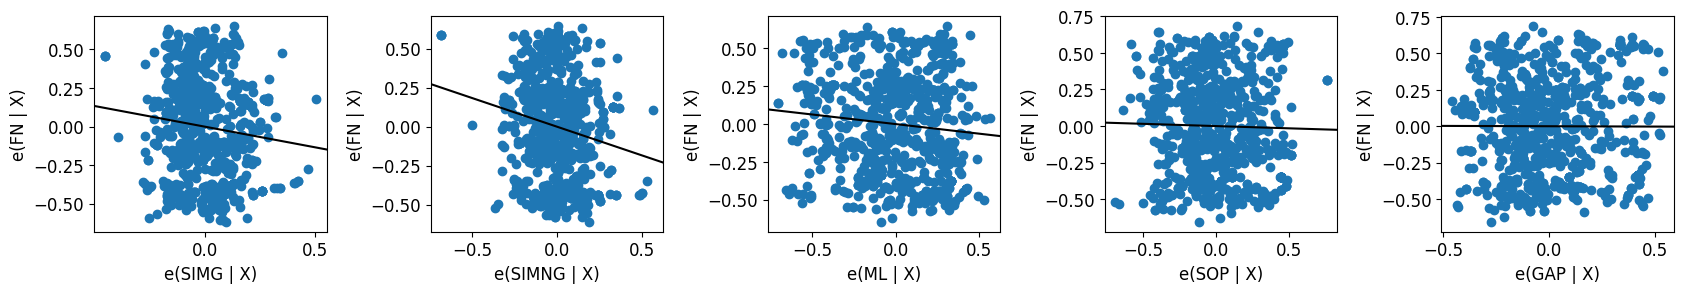
\includegraphics[width=1.1\textwidth]{partial-plot-A}}\\
\subfloat[Set B]{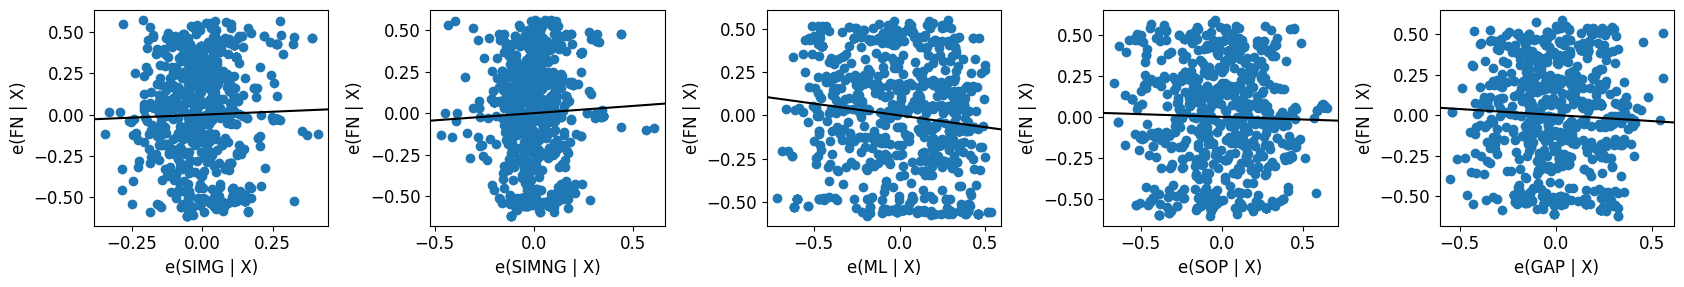
\includegraphics[width=1.1\textwidth]{partial-plot-B}}	
\end{adjustwidth}
\caption{Three sub-floats.}
\label{3figs}
\end{figure*}

\begin{figure*}[!htbp]
	\begin{adjustwidth}{-3cm}{-3cm}
		\centering
		
		\begin{subfigure}[b]{0.1\textwidth}
			\includegraphics[width=\columnwidth]{Figure/PMAO-A/BB11018-fn-ml}
			%\caption{BB11005}
			%\label{fig:con_pr09}
		\end{subfigure}    
		\begin{subfigure}[b]{0.25\textwidth}
			\includegraphics[width=\columnwidth]{Figure/PMAO-A/BB11018-fn-ml}
			%\caption{BB11018}
			%\label{fig:con_pr09}
		\end{subfigure}
		\begin{subfigure}[b]{0.25\textwidth}
			\includegraphics[width=\columnwidth]{Figure/PMAO-A/BB11018-fn-ml}
			%\caption{BB11020}
			%\label{fig:con_pr09}
		\end{subfigure}
		\begin{subfigure}[b]{0.25\textwidth}
			\includegraphics[width=\columnwidth]{Figure/PMAO-A/BB11018-fn-ml}
			%\caption{BB11033}
			%\label{fig:con_pr09}
		\end{subfigure}
		\begin{subfigure}[b]{0.25\textwidth}
			\includegraphics[width=\columnwidth]{Figure/PMAO-A/BB11018-fn-ml}
			%\caption{BB11033}
			%\label{fig:con_pr09}
		\end{subfigure}
		
		\begin{subfigure}[b]{0.25\textwidth}
			\includegraphics[width=\columnwidth]{Figure/PMAO-A/BB11018-fn-ml}
			%\caption{BB11005}
			%\label{fig:con_pr09}
		\end{subfigure}    
		\begin{subfigure}[b]{0.25\textwidth}
			\includegraphics[width=\columnwidth]{Figure/PMAO-A/BB11018-fn-ml}
			%\caption{BB11018}
			%\label{fig:con_pr09}
		\end{subfigure}
		\begin{subfigure}[b]{0.25\textwidth}
			\includegraphics[width=\columnwidth]{Figure/PMAO-A/BB11018-fn-ml}
			%\caption{BB11020}
			%\label{fig:con_pr09}
		\end{subfigure}
		\begin{subfigure}[b]{0.25\textwidth}
			\includegraphics[width=\columnwidth]{Figure/PMAO-A/BB11018-fn-ml}
			%\caption{BB11033}
			%\label{fig:con_pr09}
		\end{subfigure}
		\begin{subfigure}[b]{0.25\textwidth}
			\includegraphics[width=\columnwidth]{Figure/PMAO-A/BB11018-fn-ml}
			%\caption{BB11033}
			%\label{fig:con_pr09}
		\end{subfigure}
	
		\caption{ 3 iterations}
		\label{fig:fn_rate_3iter}
	\end{adjustwidth}
\end{figure*}
\end{comment}

